% This file was generated with po4a. Translate the source file.
%
\documentclass[10pt,table,dvipsnames,compress]{beamer}
\usepackage[utf8]{inputenc}
\usepackage[T1]{fontenc}
\usepackage{graphicx}
\usepackage{longtable}
\usepackage{wrapfig}
\usepackage{rotating}
\usepackage[normalem]{ulem}
\usepackage{amsmath}
\usepackage{amssymb}
\usepackage{capt-of}
\usepackage{hyperref}
\usetheme{default} \useinnertheme{rounded}
\useoutertheme[subsection=false]{miniframes} \date{} \title{Usar el plugin
QGIS deforisk para elaborar y comparar mapas de riesgo de deforestación}
\title[plugin QGIS deforisk]{Usar el plugin QGIS \texttt{deforisk} para
elaborar y comparar mapas de riesgo de deforestación}
\definecolor{darkgreen}{RGB}{34,139,34} \usepackage{float}
\usepackage{lmodern} \usepackage{pgf} \usepackage{color}
\usepackage[english,french]{babel} \definecolor{vertmoyen}{RGB}{51,110,23}
\definecolor{blueFRB}{HTML}{31859c} \usecolortheme[named=blueFRB]{structure}
\usepackage{tabularx} \usepackage{layout} \setlength{\LTleft}{-5cm plus 1
fill} \setlength{\LTright}{-5cm plus 1 fill} \usepackage{booktabs}
\usepackage{arydshln} \newcommand{\logit}{\text{logit}}
\newcommand{\bs}[1]{\boldsymbol{#1}}
\newcommand{\R}{\textnormal{\sffamily\bfseries R}}
\newcommand{\pkg}[1]{{\fontseries{b}\selectfont #1}}
\newcolumntype{C}[1]{>{\centering\arraybackslash}m{#1}}

\setbeamertemplate{footline}[frame number]
\setbeamertemplate{frametitle}{\usebeamerfont{frametitle}\insertframetitle\vphantom{g}
\par \centering 
\includegraphics[width=\textwidth]{figs/Barre_couleur} }
\beamertemplatenavigationsymbolsempty

\newif\ifplacelogo
\logo{\ifplacelogo
\includegraphics[width=0.5\textwidth]{figs/partners_logos}\fi}

\AtBeginSection[]{ \placelogotrue \begin{frame} \frametitle{Contenido}
\begin{columns}[c] \begin{column}{0.5\textwidth}
\tableofcontents[sections=1,currentsection] \vspace{0.5cm}
\tableofcontents[sections=2,currentsection] \vspace{0.5cm}
\tableofcontents[sections=3,currentsection] \end{column}
\begin{column}{0.5\textwidth} \tableofcontents[sections=4,currentsection]
\vspace{0.5cm} \tableofcontents[sections=5,currentsection] \end{column}
\end{columns} \end{frame} \placelogofalse }

\AtBeginSubsection[]{ \placelogotrue \begin{frame} \frametitle{Contenido}
\begin{columns}[c] \begin{column}{0.5\textwidth}
\tableofcontents[sections=1,currentsection, currentsubsection]
\vspace{0.5cm} \tableofcontents[sections=2,currentsection,
currentsubsection] \vspace{0.5cm}
\tableofcontents[sections=3,currentsection, currentsubsection] \end{column}
\begin{column}{0.5\textwidth} \tableofcontents[sections=4,currentsection,
currentsubsection] \vspace{0.5cm}
\tableofcontents[sections=5,currentsection, currentsubsection] \end{column}
\end{columns} \end{frame} \placelogofalse }

\hypersetup{
colorlinks=true, linkcolor=Black, filecolor=Maroon, citecolor=Blue,
urlcolor=Maroon}

\urlstyle{same}

\hypersetup{
 pdfauthor={Ghislain Vieilledent}, pdftitle={Usar el plugin QGIS deforisk
para elaborar y comparar mapas de riesgo de deforestación}, pdfkeywords={},
pdfsubject={}, pdfcreator={Emacs 29.3 (Org mode 9.6.15)}, pdflang={Español}}
\begin{document}



{ \setbeamertemplate{navigation symbols}{} \begin{frame}[plain,
noframenumbering] \begin{center} \small{\textbf{Taller FAO -- Santa Marta
(Colombia), Julio 2024}} \end{center} \vspace{-0.5cm} \titlepage
\vspace{-3cm} \begin{center}

\includegraphics[width=\textwidth]{figs/Barre_couleur} \vspace{0.25cm}
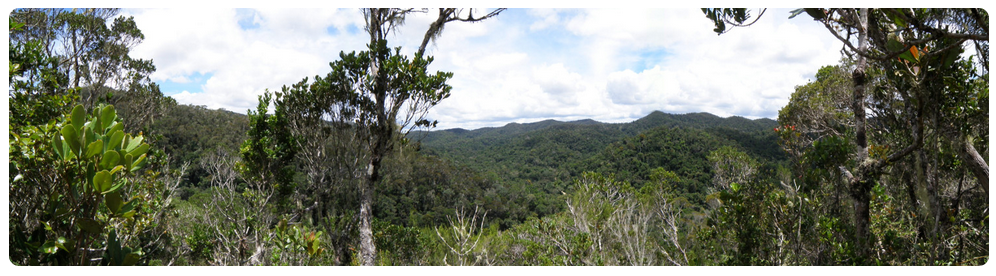
\includegraphics[width=10cm]{figs/Banniere} \small{Ghislain
VIEILLEDENT$^{1}$\hspace{0.25cm}Thomas ARSOUZE$^{1}$\hspace{0.25cm}Equipo
FAO$^{2}$} \vspace{0.25cm} {\scriptsize \begin{tabular}{l} $[1]$
\textbf{Cirad} UMR AMAP, $[2]$ \textbf{FAO} Roma y America
Latina\end{tabular} }

\includegraphics[width=0.8\textwidth]{figs/partners_logos} \end{center}
\end{frame} }


\placelogotrue
\begin{frame}
  \frametitle{Contenido}
  \begin{columns}[c]
    \begin{column}{0.5\textwidth} \tableofcontents[sections=1] \vspace{0.5cm}
\tableofcontents[sections=2] \vspace{0.5cm} \tableofcontents[sections=3]
    \end{column}
    \begin{column}{0.5\textwidth} \tableofcontents[sections=4] \vspace{0.5cm}
\tableofcontents[sections=5]
    \end{column}
  \end{columns}
\end{frame}
\placelogofalse

\section{El plugin QGIS deforisk}
\label{sec:org33875a8}

\subsection{Objetivo y especificidades}
\label{sec:org2b48526}

\begin{frame}[label={sec:org9b9dfa0}]{Objetivos}
\begin{itemize}
\item Proporcionar \textbf{una herramienta} para elaborar y comparar \textbf{mapas
de riesgo de deforestación}.
\item Al nivel \textbf{jurisdictional}.
\item Siguiendo la \textbf{metodología de Verra} para la certificación.
\item \textbf{Asignar la deforestación} a proyectos dentro de la jurisdicción.
\end{itemize}
\end{frame}

\begin{frame}[label={sec:org670f662}]{Especificidades}
\begin{itemize}
\item De código abierto y basado en Python: transparencia, reproducibilidad.
\item Cálculos rápidos:
\begin{itemize}
\item Procesamiento de rasters por bloques.
\item Ejecución de tareas en paralelo.
\end{itemize}
\item Independiente del sistema operativo: Windows, Linux, MacOS.
\item Debería funcionar en cualquier ordenador con un rendimiento medio.
\item Modelos estadísticos alternativos eficaces (iCAR).
\item Totalmente documentado y traducido (inglés, español, francés).
\item Ayuda en la preparación de datos.
\item Debería ser (relativamente) fácil de usar.
\end{itemize}
\end{frame}

\begin{frame}[label={sec:orgad092f5},fragile]{Basado sobre Python}
 El plugin \texttt{deforisk} se basa en cuatro paquetes de Python
desarrollados específicamente para modelar la deforestación:

\begin{itemize}
\item \texttt{geefcc}: realizar mapas de cambios en la cubierta forestal a partir
de Google Earth Engine (GEE).
\item \texttt{pywdpa}: descarga de áreas protegidas de la Base de Datos Mundial
sobre Áreas Protegidas (WDPA).
\item \texttt{forestatrisk}: modelizar la deforestación y predecir la
deforestación espacial.
\item \texttt{riskmapjnr}: mapas de riesgo según las metodologías Verra JNR.
\end{itemize}

\begin{center}
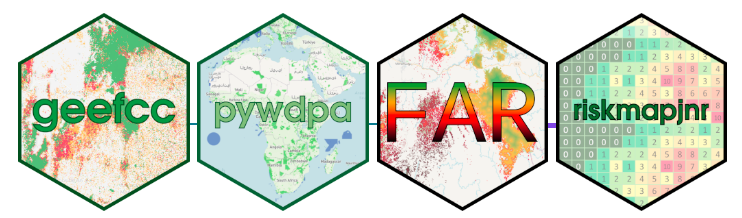
\includegraphics[width=0.7\textwidth]{figs/logos-packages.png}
\end{center}
\end{frame}

\begin{frame}[label={sec:org3f9636c},fragile]{Procesamiento de rasters por bloques.}
 \begin{itemize}
\item Los archivos raster de cambio de cubierta forestal y las variables
explicativas pueden ocupar un espacio de varios gigabytes en disco.
\item El procesamiento en memoria de rasters tan grandes puede ser imposible en
ordenadores con una memoria RAM limitada.
\item Las funciones utilizadas en el plugin \texttt{deforisk} procesan grandes
rásters por bloques de píxeles que representan subconjuntos de los datos
ráster.
\item Esto hace que el cálculo sea eficiente, con un bajo uso de memoria.
\end{itemize}

\begin{center}
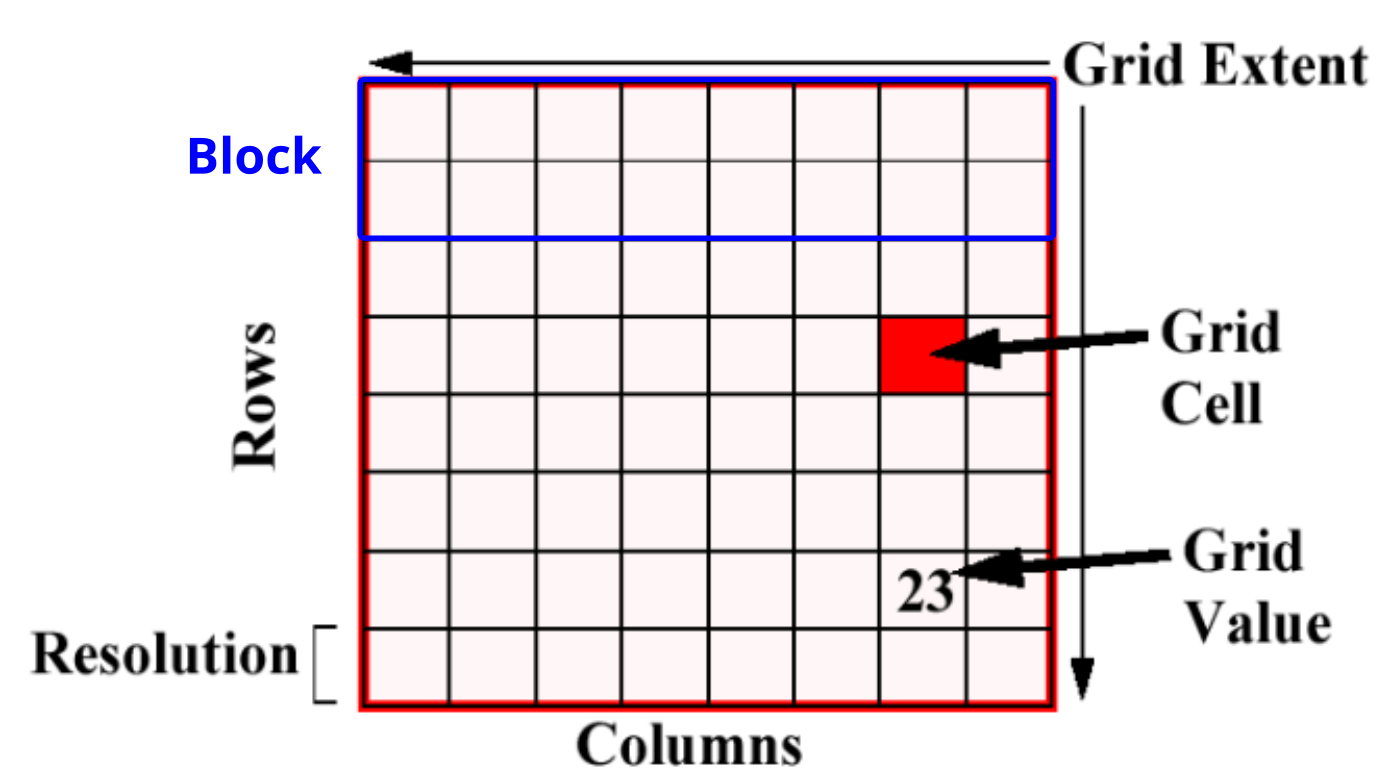
\includegraphics[width=6cm]{figs/raster_block.png}
\end{center}
\end{frame}

\begin{frame}[label={sec:org87726f7},fragile]{Ejecución de tareas en paralelo.}
 \begin{itemize}
\item El enfoque más avanzado para seleccionar el mejor mapa de riesgos implica
repetir tareas (modelo, periodos).
\item Para ahorrar tiempo de cálculo, el plugin \texttt{deforisk} utiliza el
gestor de tareas de QGIS.
\item Permite ejecutar varios análisis en paralelo.
\end{itemize}

\vspace{0.25cm}

\begin{center}
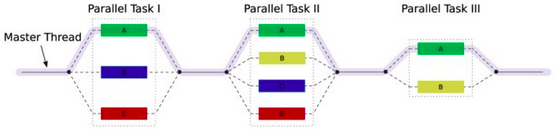
\includegraphics[width=9cm]{figs/parallel_tasks.png}
\end{center}
\end{frame}

\subsection{Sitio web y documentación}
\label{sec:orgd6a1b3f}

\begin{frame}[label={sec:orgb622ffa}]{Sitio web y documentación}
El sitio web incluye toda la documentación para utilizar el plugin:

\begin{itemize}
\item \href{https://deforisk-qgis-plugin.org/es/installation.html}{Página de
instalación}: ¿Cómo instalar el plugin?
\item \href{https://deforisk-qgis-plugin.org/es/plugin\_api.html}{Página API del
plugin}: ¿Cuál es el significado de cada parámetro?
\item \href{https://deforisk-qgis-plugin.org/es/get_started.html}{Página de
inicio}. Cómo empezar a utilizar el plugin en una pequeña área de interés?
\item \href{https://deforisk-qgis-plugin.org/es/articles.html}{Página de
artículos}. Cómo puedo utilizar el plugin para casos específicos
(jurisdicciones subnacionales, datos del usuario)?
\item \href{https://deforisk-qgis-plugin.org/es/articles/references.html}{Referencias}:
Una página con documentos de referencia, incluidas presentaciones.
\end{itemize}

\begin{columns}
\begin{column}{0.5\columnwidth} \flushright \url{https://deforisk-qgis-plugin.org}
\end{column}
\begin{column}{0.5\columnwidth}
\begin{center}
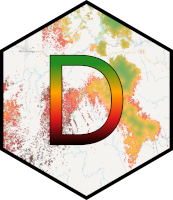
\includegraphics[width=2cm]{figs/logo-deforisk.png}
\end{center}
\end{column}
\end{columns}
\end{frame}

\subsection{Instalación}
\label{sec:org724424f}

\begin{frame}[label={sec:org540feec},fragile]{Instalación}
 Bajo número de pasos para instalar el plugin:

\begin{itemize}
\item Instale QGIS y GDAL en su sistema (utilizando \texttt{OSGeo4W} en Windows).
\item Instale los paquetes de Python \texttt{forestatrisk} y \texttt{riskmapjnr}
utilizando pip.
\item \href{https://github.com/ghislainv/deforisk-qgis-plugin/archive/refs/heads/main.zip}{Descargar}
e instalar el plugin \texttt{deforisk} de QGIS.
\item (Sólo sistemas tipo Unix: instalar herramientas OSM).
\end{itemize}

\begin{center}
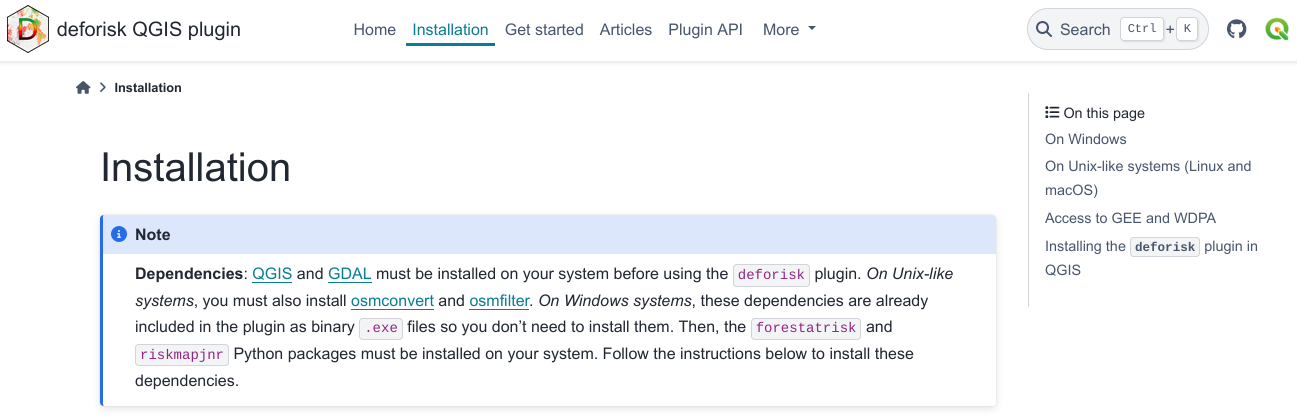
\includegraphics[width=0.9\textwidth]{figs/installation.png}
\end{center}
\end{frame}

\section{Preparación de datos}
\label{sec:org43b0b1c}

\subsection{Obtener variables}
\label{sec:org4540d1c}

\begin{frame}[label={sec:orgf7a27fd}]{Obtener variables}
\begin{columns}
\begin{column}{0.5\columnwidth}
\begin{itemize}
\item Funciones que ayudan a preparar los datos para la modelización de la
deforestación.
\item Dos fuentes diferentes para \textbf{cambio en la cubierta forestal} (GFC o
TMF).
\item Variables explicativas espaciales que describen la \textbf{accesibilidad a
los bosques} y la \textbf{tenencia de la tierra} (altitud, pendiente,
distancia a carreteras, zonas protegidas, etc.).
\end{itemize}
\end{column}

\begin{column}{0.5\columnwidth}
\begin{center}
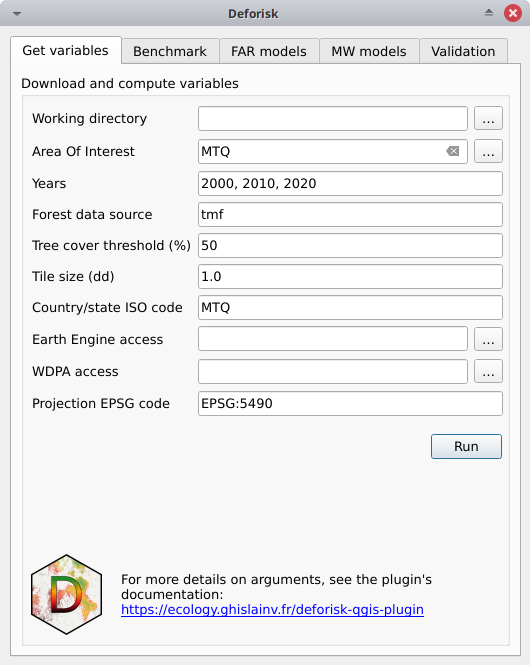
\includegraphics[width=5cm]{figs/plugin_api/interface_variables.png}
\end{center}
\end{column}
\end{columns}
\end{frame}

\subsection{Datos sobre cambios en la cubierta forestal}
\label{sec:org7f33108}

\begin{frame}[label={sec:orgaeedc82}]{Datos de GFC}
\begin{itemize}
\item Hansen et al.  2013.
\item Conjunto de datos global que abarca todos los tipos de bosque.
\item Cubierta arbórea y pérdida anual de cubierta arbórea.
\item Resolución de 30 m, a partir de 2000.
\item Datos: \url{https://glad.earthengine.app/view/global-forest-change}
\end{itemize}

\begin{center}
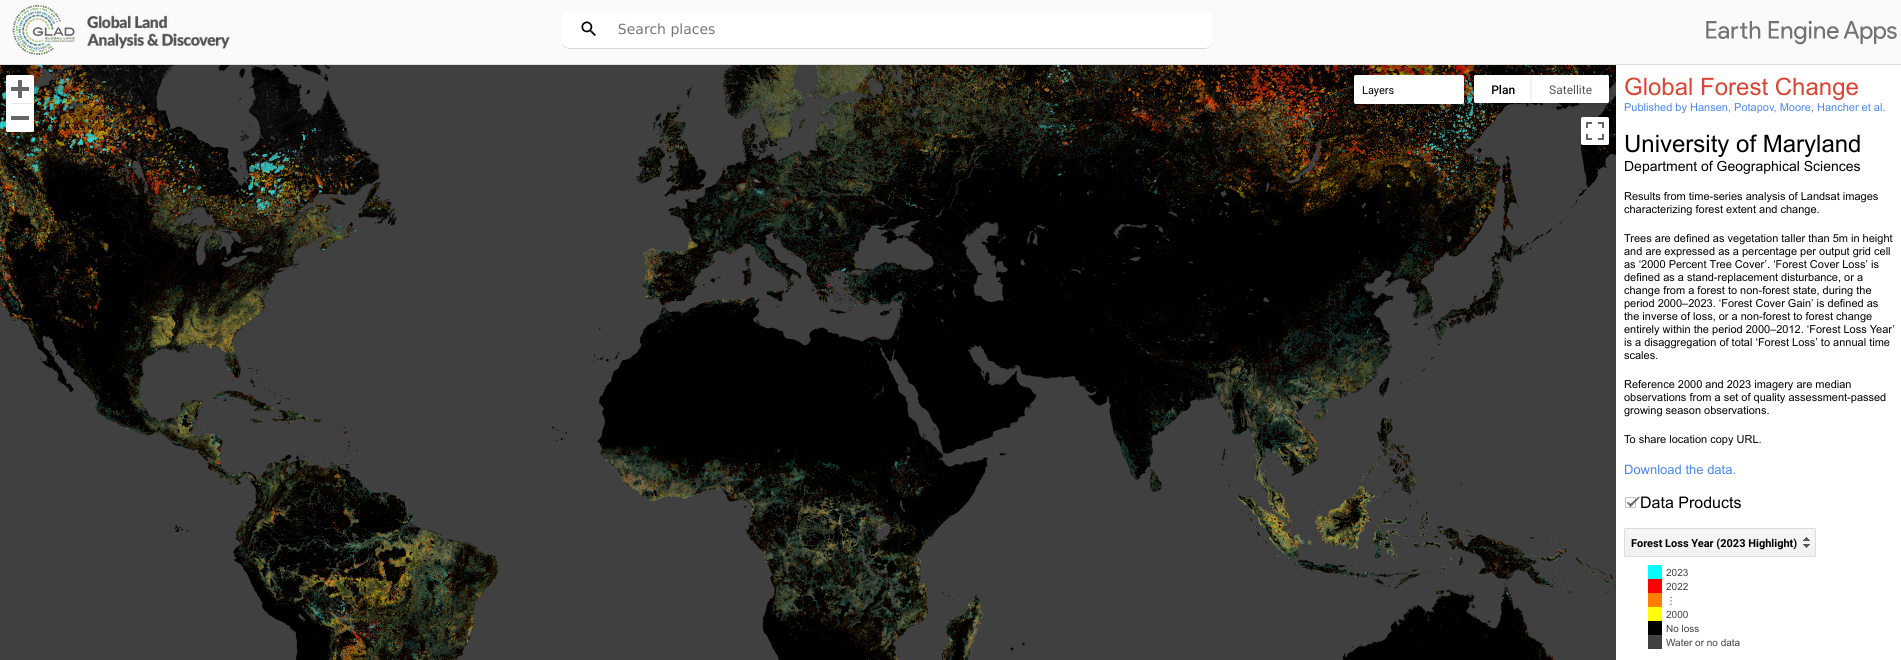
\includegraphics[width=\textwidth]{figs/gfc.png}
\end{center}
\end{frame}

\begin{frame}[label={sec:org4f33ca0}]{Datos de TMF}
\begin{itemize}
\item Vancutsem et al.  2021.  Bosques húmedos tropicales (bosque perennifolio, no
hay bosques caducifolios secos).
\item Resolución de 30 m, a partir de 1990.
\item La deforestación tropical se subestimó (-33\% en 2000--2012, Hansen et al. 
2013), especialmente en África.
\item Datos: \url{https://forobs.jrc.ec.europa.eu/TMF/}.
\end{itemize}

\vspace{0.25cm}

\begin{center}
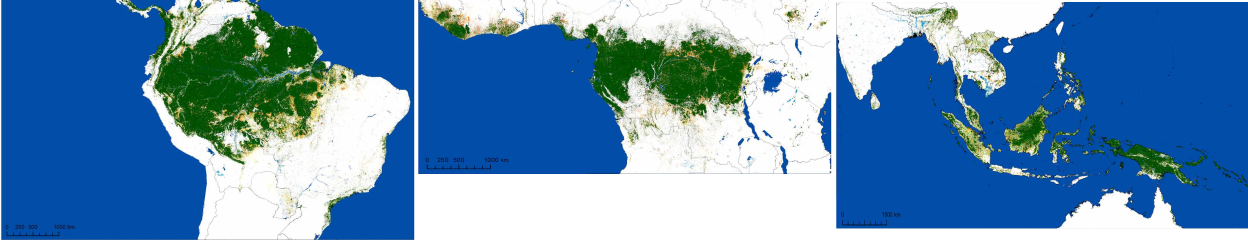
\includegraphics[width=\textwidth]{figs/Vancutsem2021-maps-wide.png}
\end{center}
\end{frame}

\begin{frame}[label={sec:orgd0bbec4}]{Datos de TMF}
\begin{itemize}
\item Suficientemente precisos para identificar visualmente las causas de la
deforestación (tala, incendios, agricultura).
\end{itemize}

\begin{center}
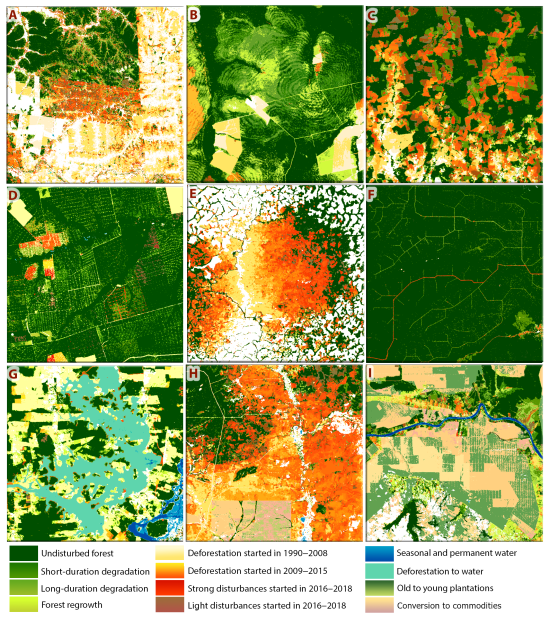
\includegraphics[width=0.5\textwidth]{figs/Vancutsem2021-patterns.png}
\end{center}
\end{frame}

\subsection{Variables explicativas espaciales}
\label{sec:org3a75228}

\begin{frame}[label={sec:org8b6e56b}]{Variables explicativas espaciales}
El plugin ayuda a calcular ocho variables explicativas.

\begin{center}
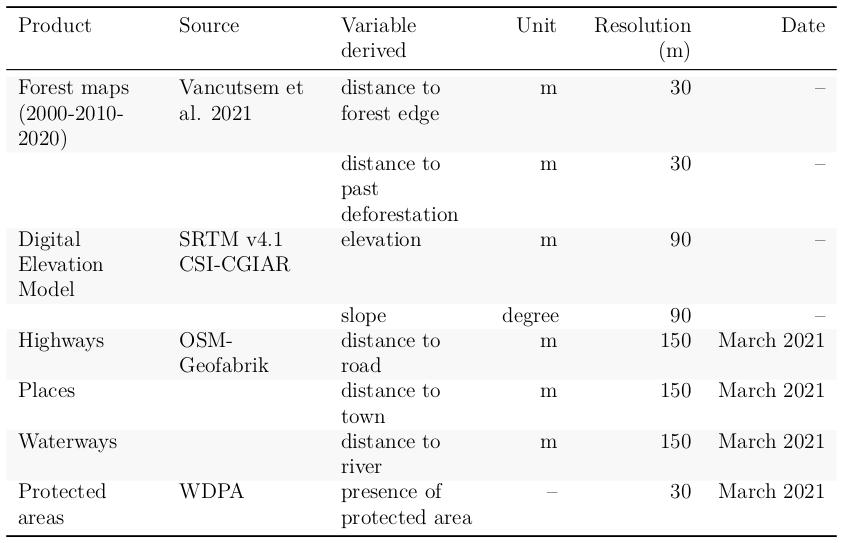
\includegraphics[width=0.75\textwidth]{figs/variables-tab.png}
\end{center}
\end{frame}

\begin{frame}[label={sec:orgbd91830}]{Variables explicativas espaciales}
\begin{center}
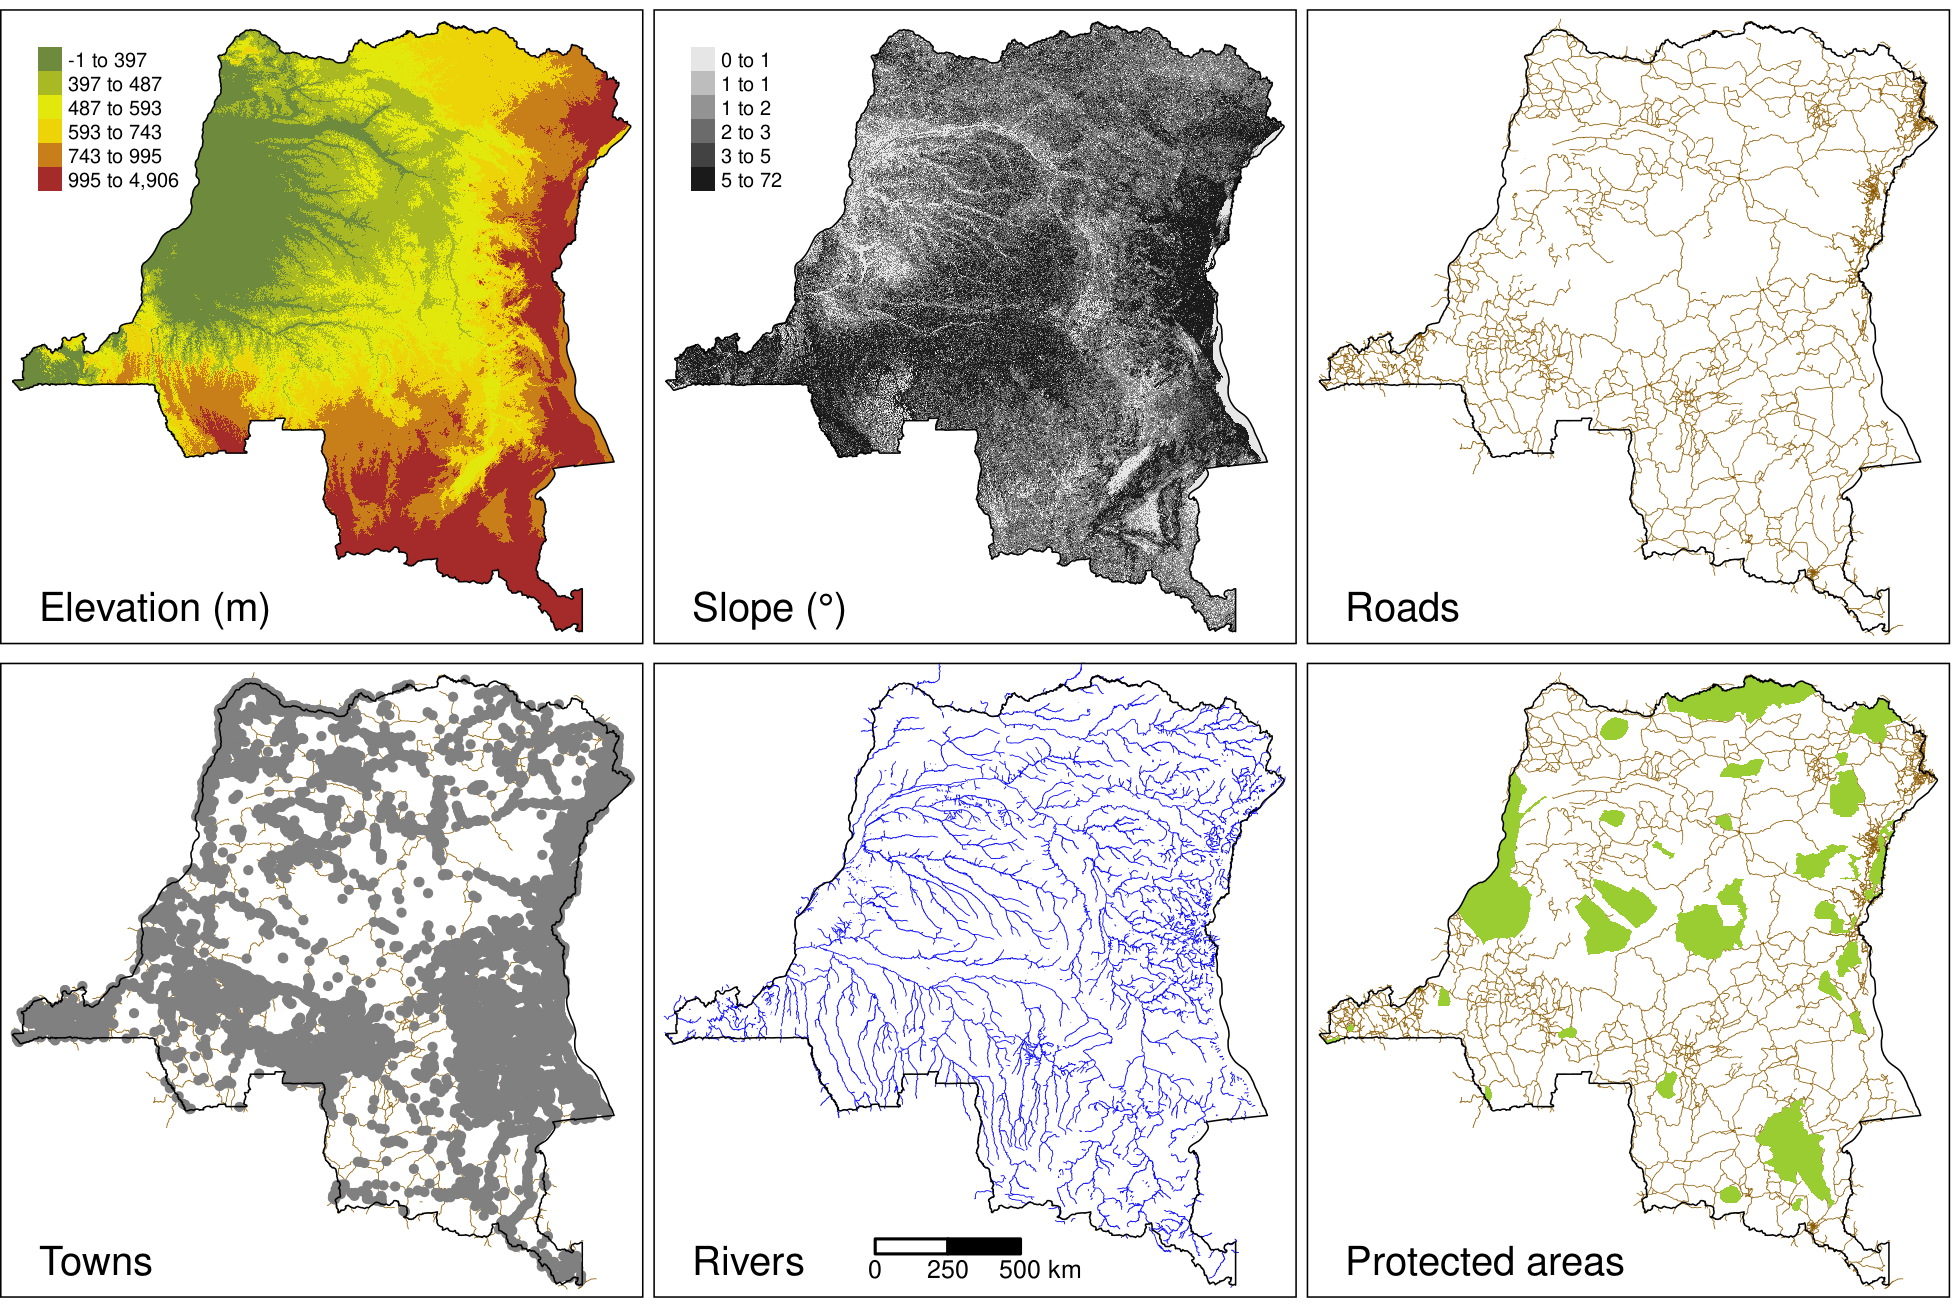
\includegraphics[width=0.8\textwidth]{figs/sm/var.png}
\end{center}

\centering \textbf{Variables explicativas espaciales en la RDC}
\end{frame}

\begin{frame}[label={sec:orgd6e5a80}]{Carreteras}
\begin{itemize}
\item OpenStreetMap (OSM)
\item ``motorway'', ``trunk'', ``primary'', ``secondary'' y ``tertiary''
carreteras
\item 3,6 millones de carreteras de OSM
\end{itemize}

\begin{center}
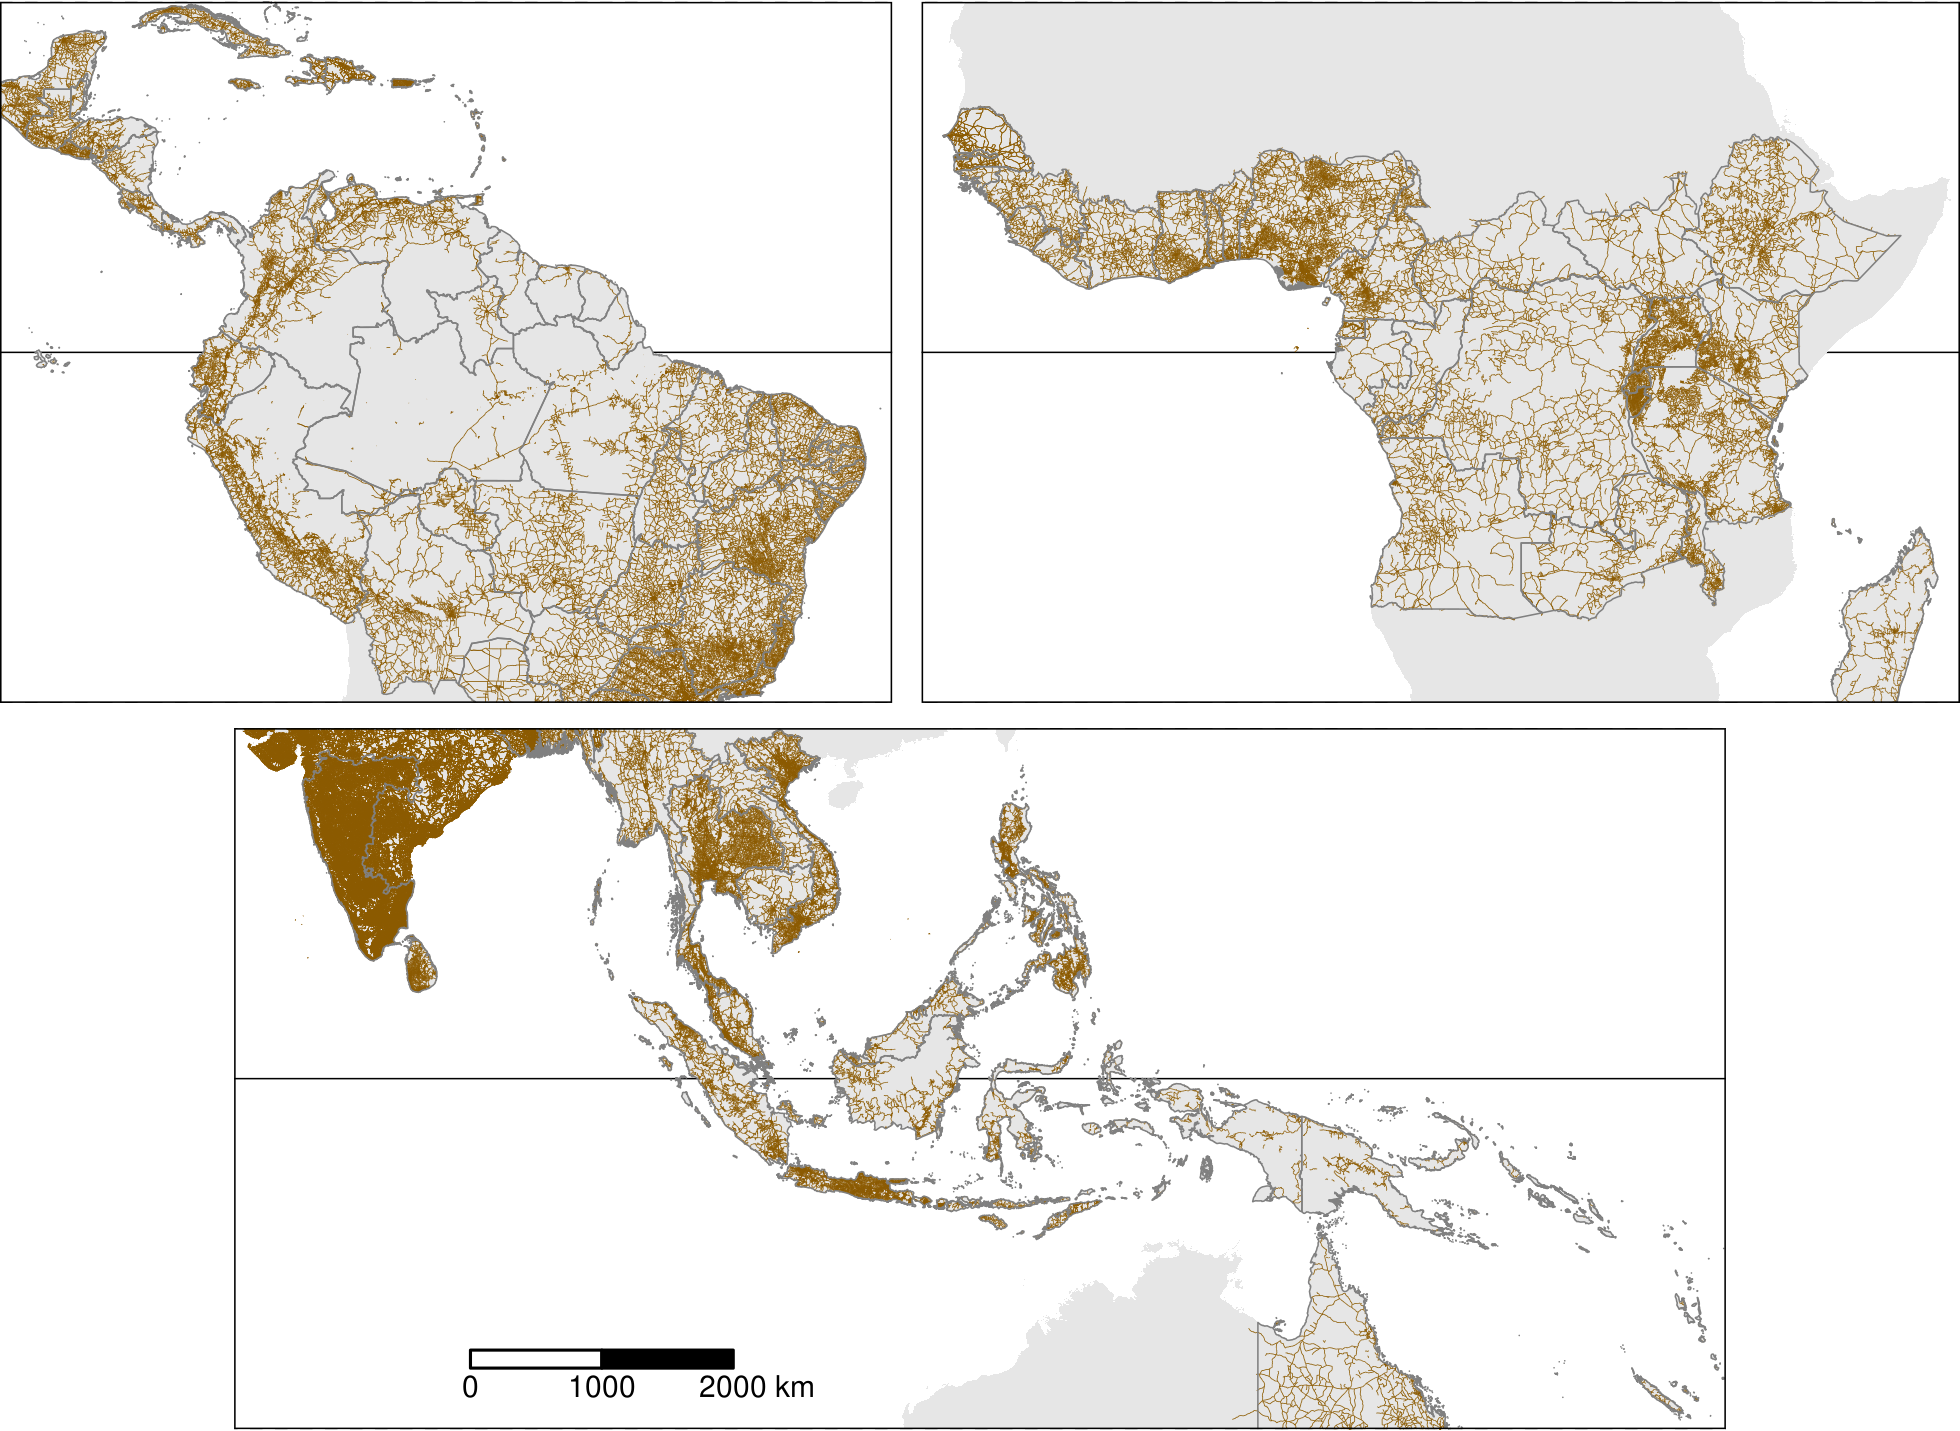
\includegraphics[width=0.7\textwidth]{figs/sm/roads.png}
\end{center}
\end{frame}

\begin{frame}[label={sec:org0304202}]{Areas protegidas}
\begin{itemize}
\item Estado de la AP: "Designada", "Inscrita", "Establecida" o "Propuesta".
\item 85.000 zonas protegidas de la WDPA.
\end{itemize}

\begin{center}
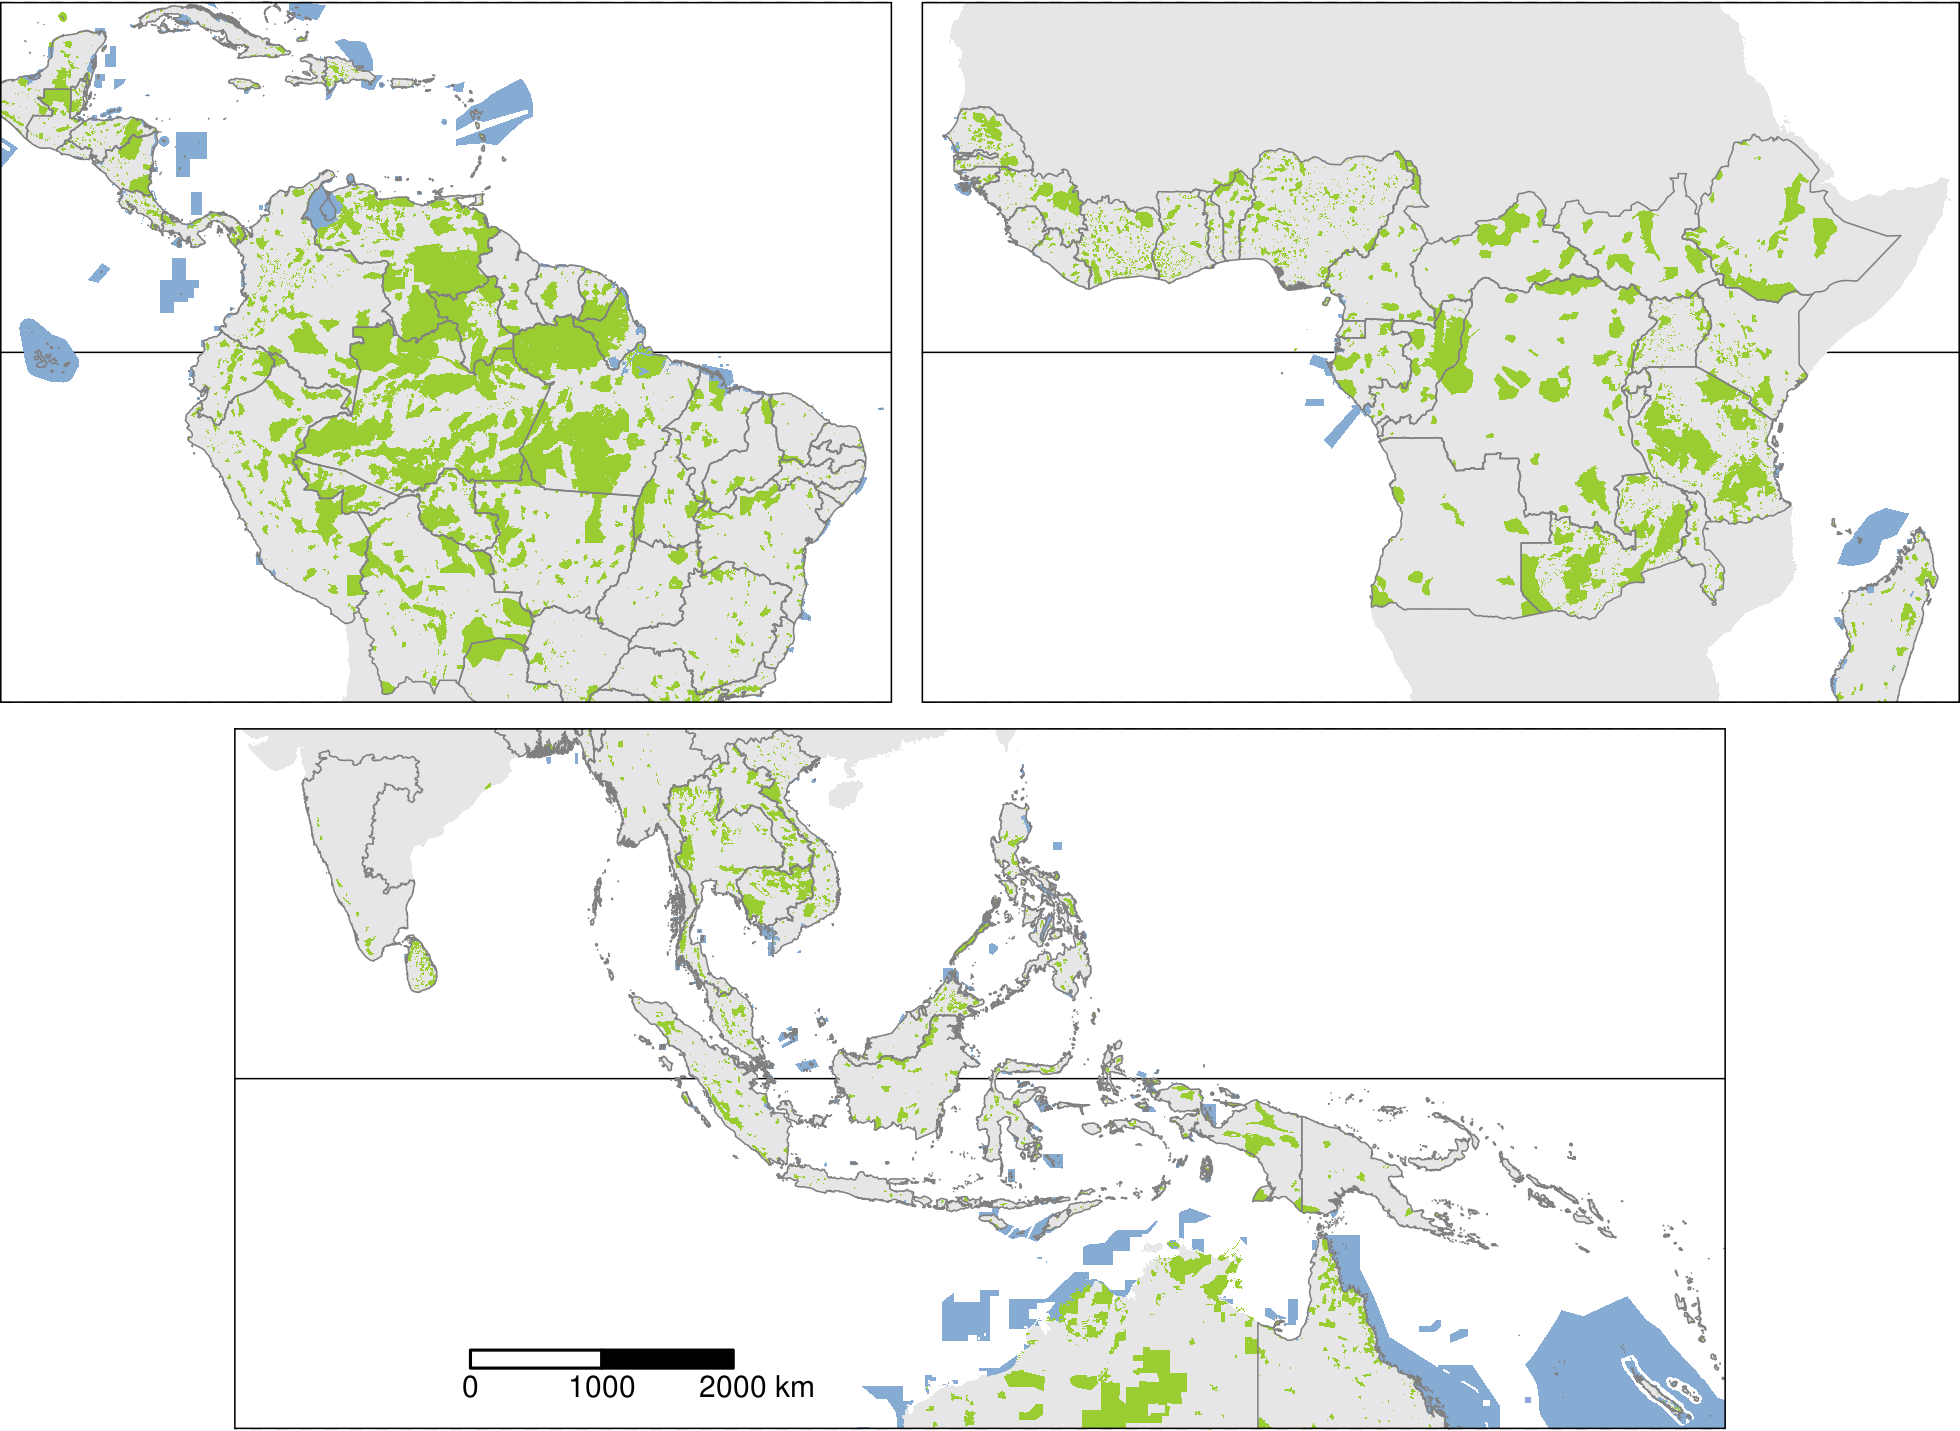
\includegraphics[width=0.7\textwidth]{figs/sm/pa.png}
\end{center}
\end{frame}

\section{Modelos y validación}
\label{sec:orge1c0621}

\subsection{Modelo de referencia}
\label{sec:org4d6d90a}

\begin{frame}[label={sec:org46860d4}]{Modelo de referencia}
\begin{columns}
\begin{column}{0.5\columnwidth}
\begin{itemize}
\item Modelo de referencia.
\item Un modelo de deforestación razonablemente bueno (mejor que un modelo nulo).
\item Asumiendo una \emph{disminución de la deforestación con la distancia al
borde del bosque} (comúnmente admitido).
\item Y un \emph{modelo diferente entre subjurisdicciones} (variabilidad
regional).
\item Ver presentación \textbf{Cirad y
FAO}.
2024.
\href{https://deforisk-qgis-plugin.org/es/\_static/references/Cirad2024-riskmap-verra.es.pdf}{Mapas
de riesgo jurisdiccional para la asignación de la deforestación}.
\end{itemize}
\end{column}

\begin{column}{0.5\columnwidth}
\begin{center}
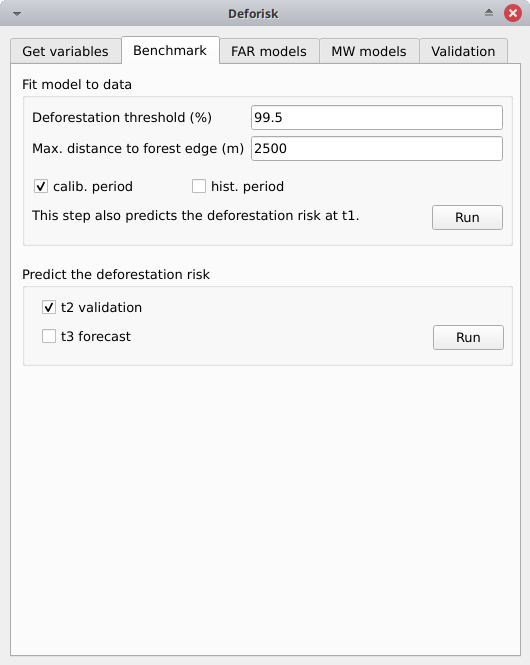
\includegraphics[width=5cm]{figs/plugin_api/interface_benchmark.png}
\end{center}  
\end{column}
\end{columns}
\end{frame}

\subsection{Modelos forestatrisk}
\label{sec:org0b990cb}

\begin{frame}[label={sec:org989b75f}]{Modelos forestatrisk}
\begin{columns}
\begin{column}{0.5\columnwidth}
\begin{itemize}
\item Tres modelos estadísticos: iCAR, GLM, RF.
\item iCAR: Regresión logística con efectos aleatorios espaciales (proceso iCAR).
\item MLG: Modelo lineal generalizado, regresión logística simple (sin efectos
aleatorios).
\item Modelo Random Forest: árboles de regresión aleatorios.
\item Modelos estadísticos basados en una muestra de las observaciones.
\end{itemize}
\end{column}

\begin{column}{0.5\columnwidth}
\begin{center}
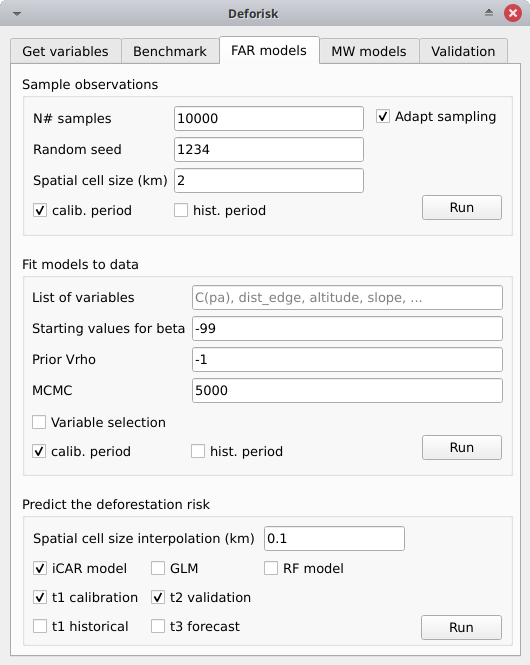
\includegraphics[width=5cm]{figs/plugin_api/interface_far_models.png}
\end{center}  
\end{column}
\end{columns}
\end{frame}

\begin{frame}[label={sec:org0bbacb1}]{Muestreo para modelos FAR}
\begin{itemize}
\item Consideramos el cambio de cubierta forestal entre \(t\) y \(t+1\).
\item Muestreo estratificado entre píxeles deforestados/no deforestados.
\item Número total de puntos proporcional a la cubierta forestal (de 20.000 a
100.000 puntos por zona de estudio).
\end{itemize}

\begin{center}
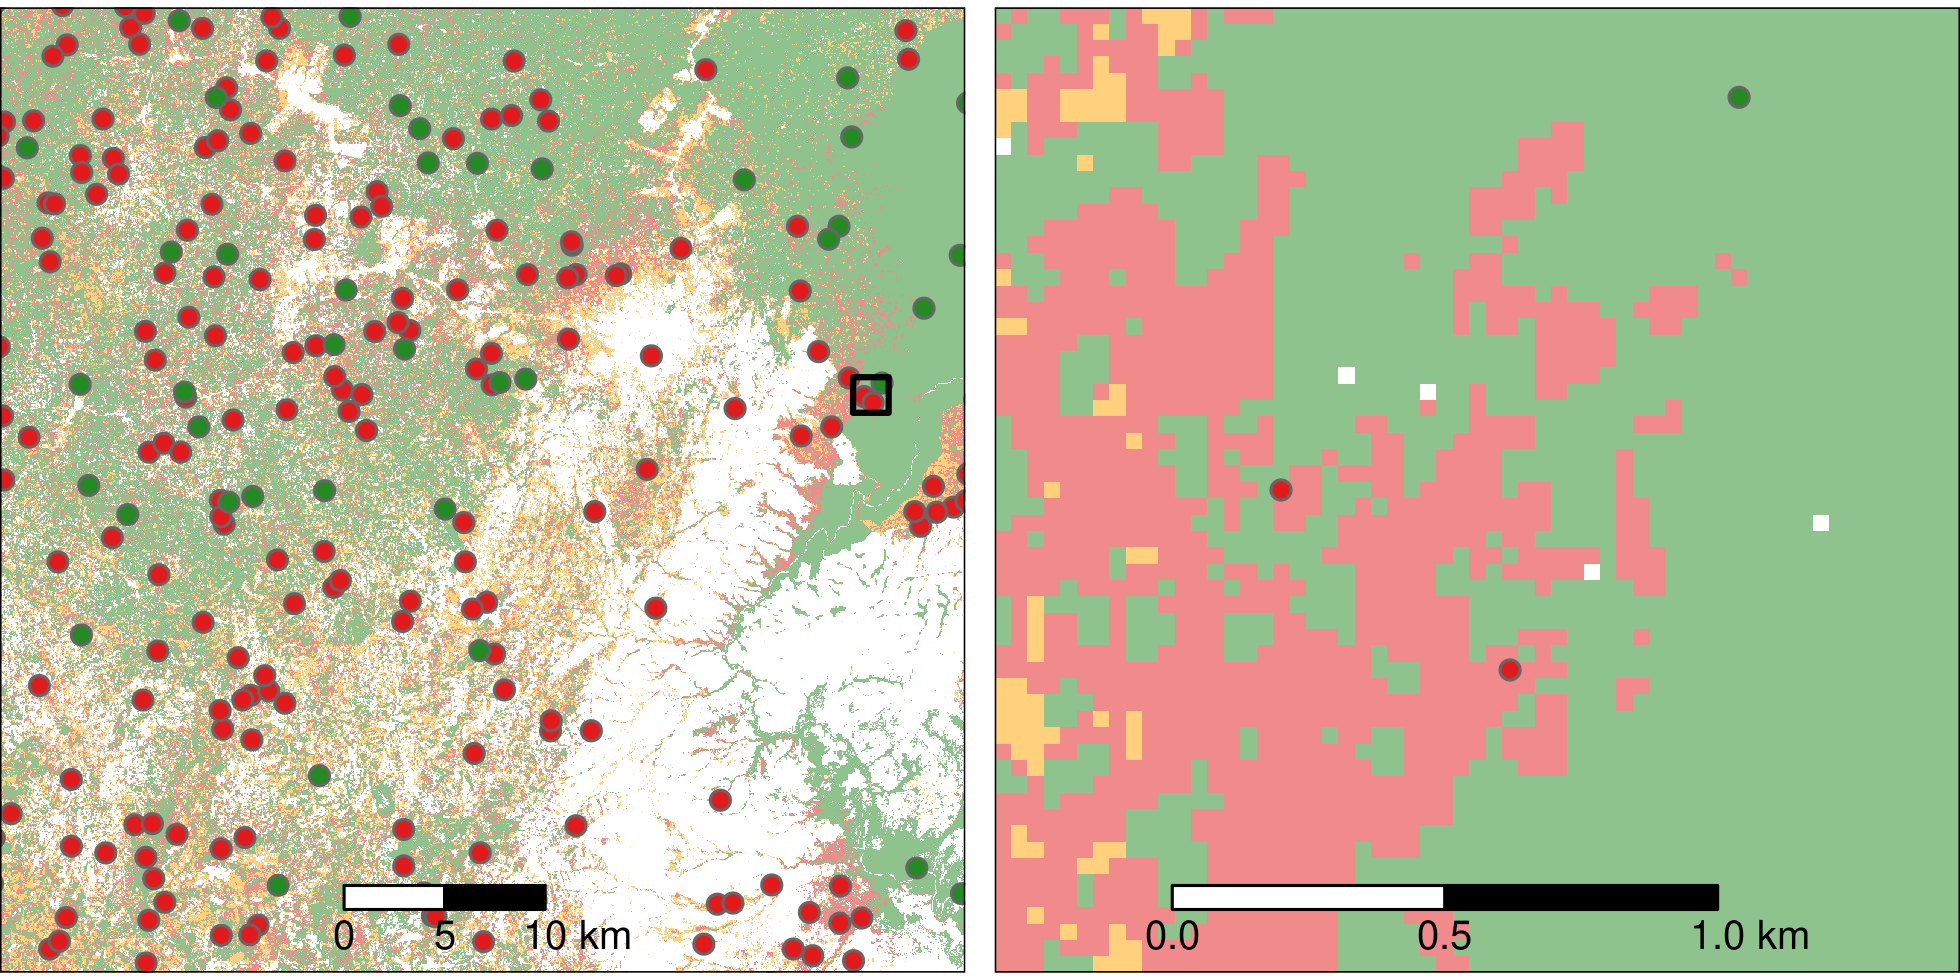
\includegraphics[width=0.7\textwidth]{figs/sm/sample.png}
\end{center}
\end{frame}

\begin{frame}[label={sec:orgd30ce3c}]{Modelo iCAR}
\begin{columns}
\begin{column}{0,5\columnwidth} Un modelo de regresión logística con proceso iCAR:

\begin{equation*}
\begin{split}
  y_i \sim \mathcal{B}ernoulli(\theta_i)\\ \text{logit}(\theta_i) = \alpha +
X_i \beta + \rho_{j(i)}\\ \rho_{j(i)} \sim
\mathcal{N}ormal(\sum_{j^{\prime}} \rho_{j^{\prime}} / n_j,V_{\rho} / n_j)
\end{split}
\end{equation*}

\textbf{Los efectos aleatorios \(\rho_{j(i)}\) permiten dar cuenta de la variación
espacial residual no tenida en cuenta por las variables del modelo \(X_i\).}
\end{column}

\begin{column}{0.5\columnwidth}
\begin{center}
\includegraphics[width=\textwidth]{figs/sm/grid.png}
\end{center}

\centering \textbf{Cuadrícula cuadrada de 10 km sobre la RDC}
\end{column}
\end{columns}
\end{frame}

\begin{frame}[label={sec:orge7256cf}]{Efectos aleatorios espaciales}
\begin{center}
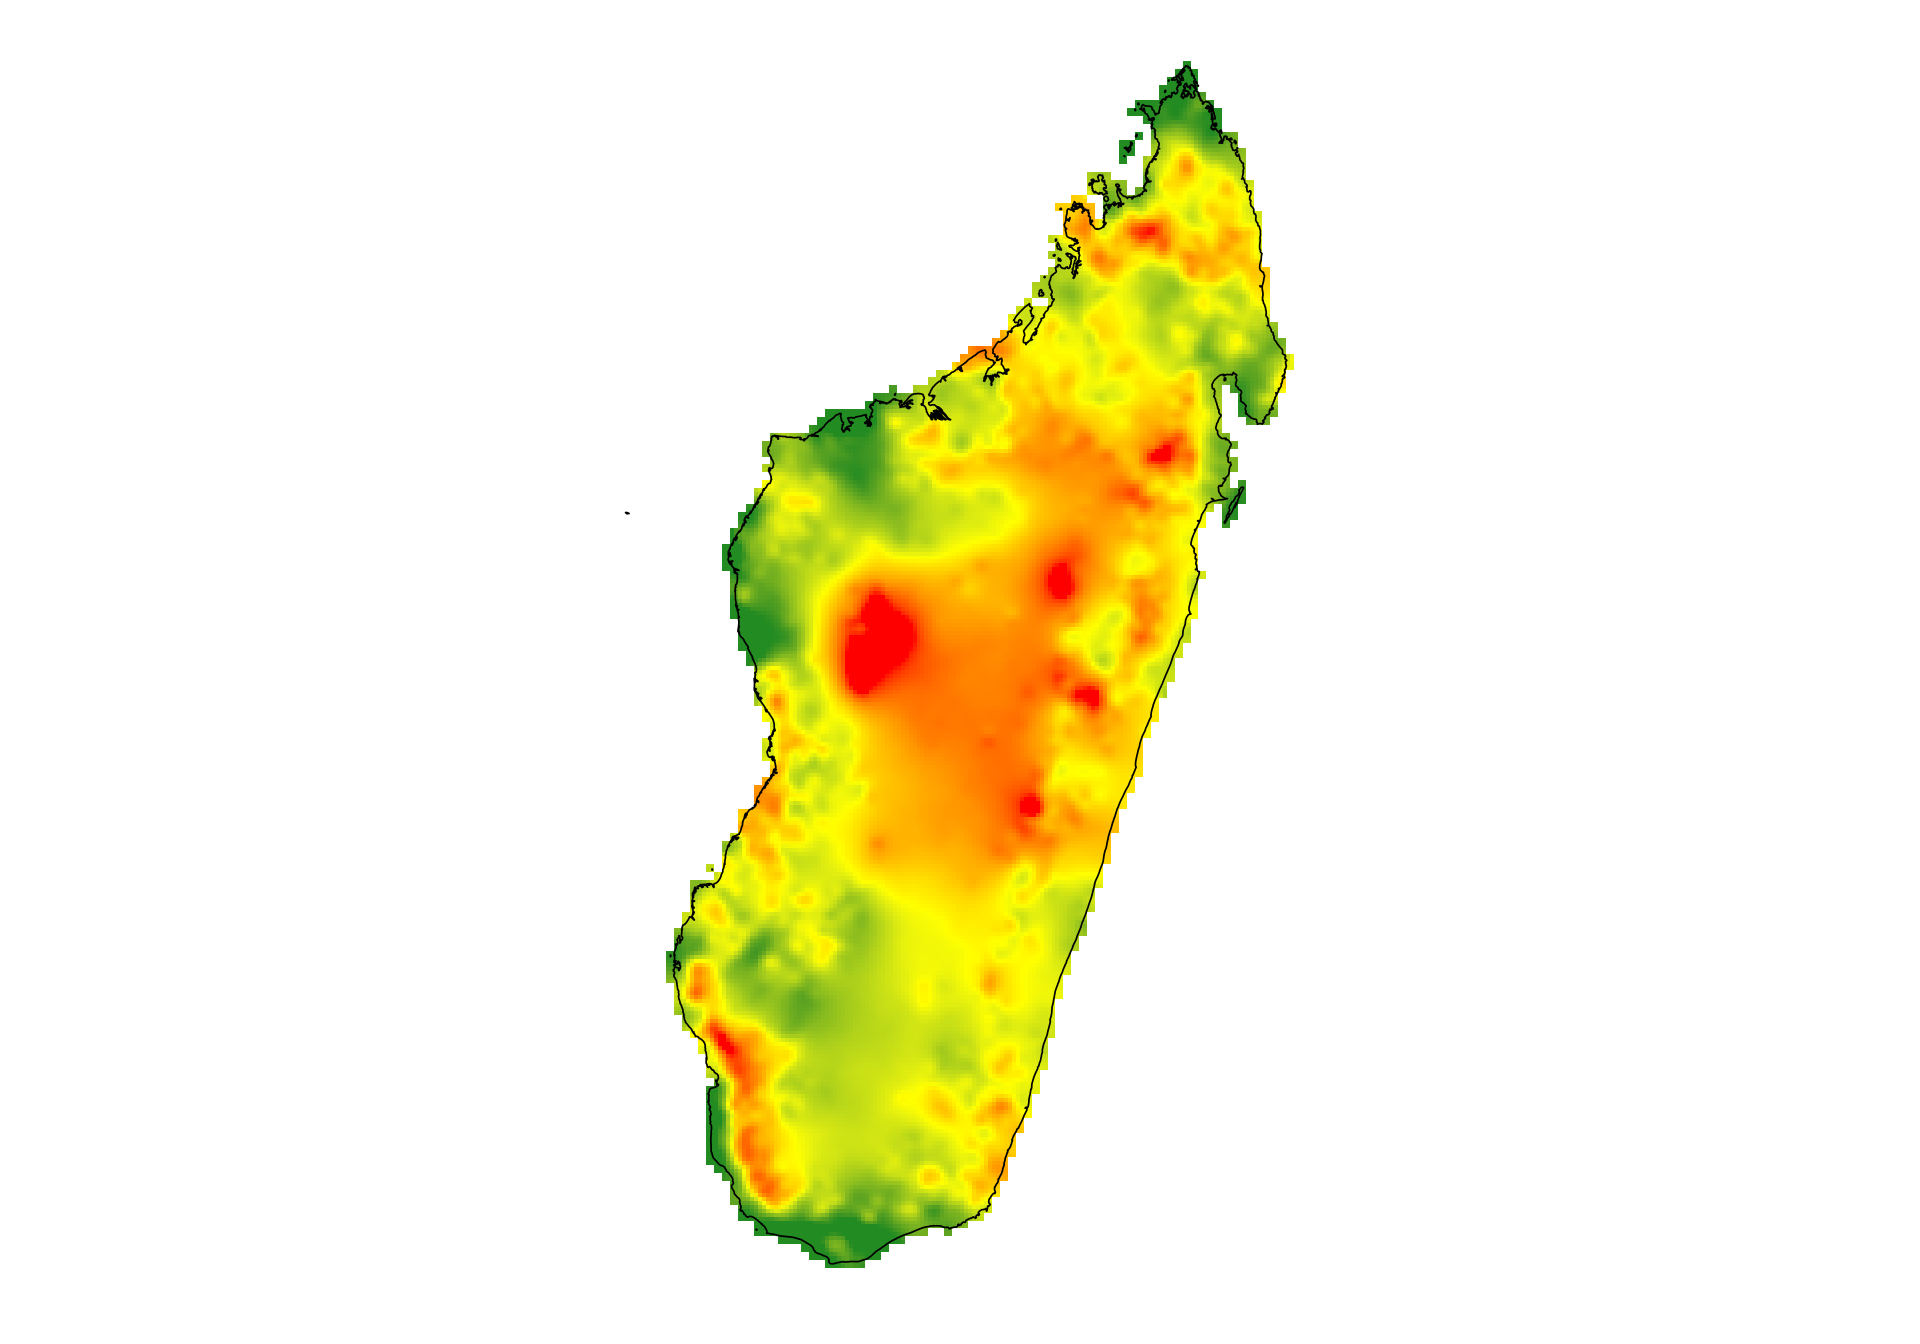
\includegraphics[width=0.6\textwidth]{figs/sm/rho.png}
\end{center}

\centering \textbf{Interpolación de efectos aleatorios espaciales a 1 km en la RDC}
\end{frame}

\begin{frame}[label={sec:org0f0fda3}]{Probabilidad espacial relativa de deforestación}
\begin{itemize}
\item Utilizamos el modelo ajustado para calcular la probabilidad espacial de
deforestación
\item Las probabilidades en [0, 1] se transforman en clases [1, 65535].
\end{itemize}

\begin{center}
\includegraphics[width=0.5\textwidth]{figs/sm/prob.png}
\end{center}

\centering \textbf{Probabilidad espacial relativa de deforestación en la RDC}
\end{frame}

\begin{frame}[label={sec:org599fb42}]{Modelo GLM}
Un modelo de regresión logística simple sin efectos aleatorios:

\begin{equation*}
\begin{split}
  y_i \sim \mathcal{B}ernoulli(\theta_i)\\texto{logit}(\theta_i) = \alpha +
X_i \beta
\end{split}
\end{equation*}

Fácil de comparar con iCAR para ver el impacto de los efectos aleatorios
espaciales.
\end{frame}

\begin{frame}[label={sec:org52dbe2f}]{Modelo Random Forest}
\begin{itemize}
\item Random Forest es un algoritmo de aprendizaje automático por conjuntos.
\item Combina varios árboles de decisión para crear un modelo predictivo más
sólido y preciso.
\end{itemize}

\begin{center}
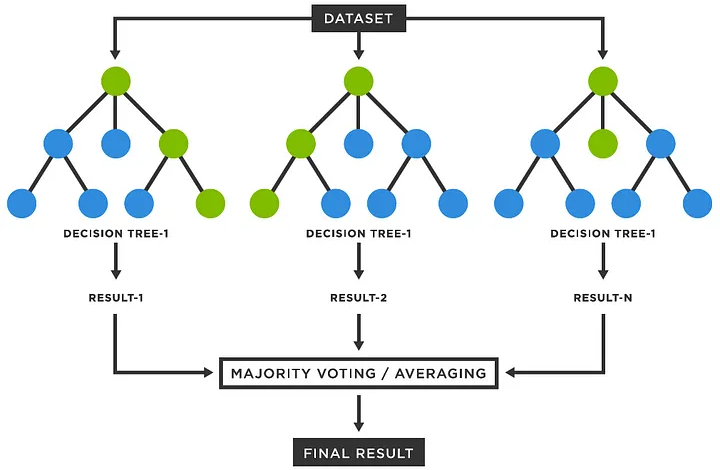
\includegraphics[width=0.7\textwidth]{figs/random_forest.png}
\end{center}
\end{frame}

\begin{frame}[label={sec:orgd707d4f}]{ForestAtRisk en los trópicos}
\begin{itemize}
\item \textbf{i.} Considerar el bosque húmedo tropical en \textbf{92} países (119
áreas de estudio).
\item \textbf{ii.} Estimar la tasa de deforestación actual y la incertidumbre en
cada país
\item \textbf{iii.} Modelizar el riesgo espacial de deforestación a partir de
factores medioambientales
\item \textbf{iv.} Previsión de la deforestación suponiendo un escenario sin
cambios
\item \textbf{v.} Consecuencias en términos de emisiones de carbono
\end{itemize}

\vspace{0.5cm}
\begin{center}
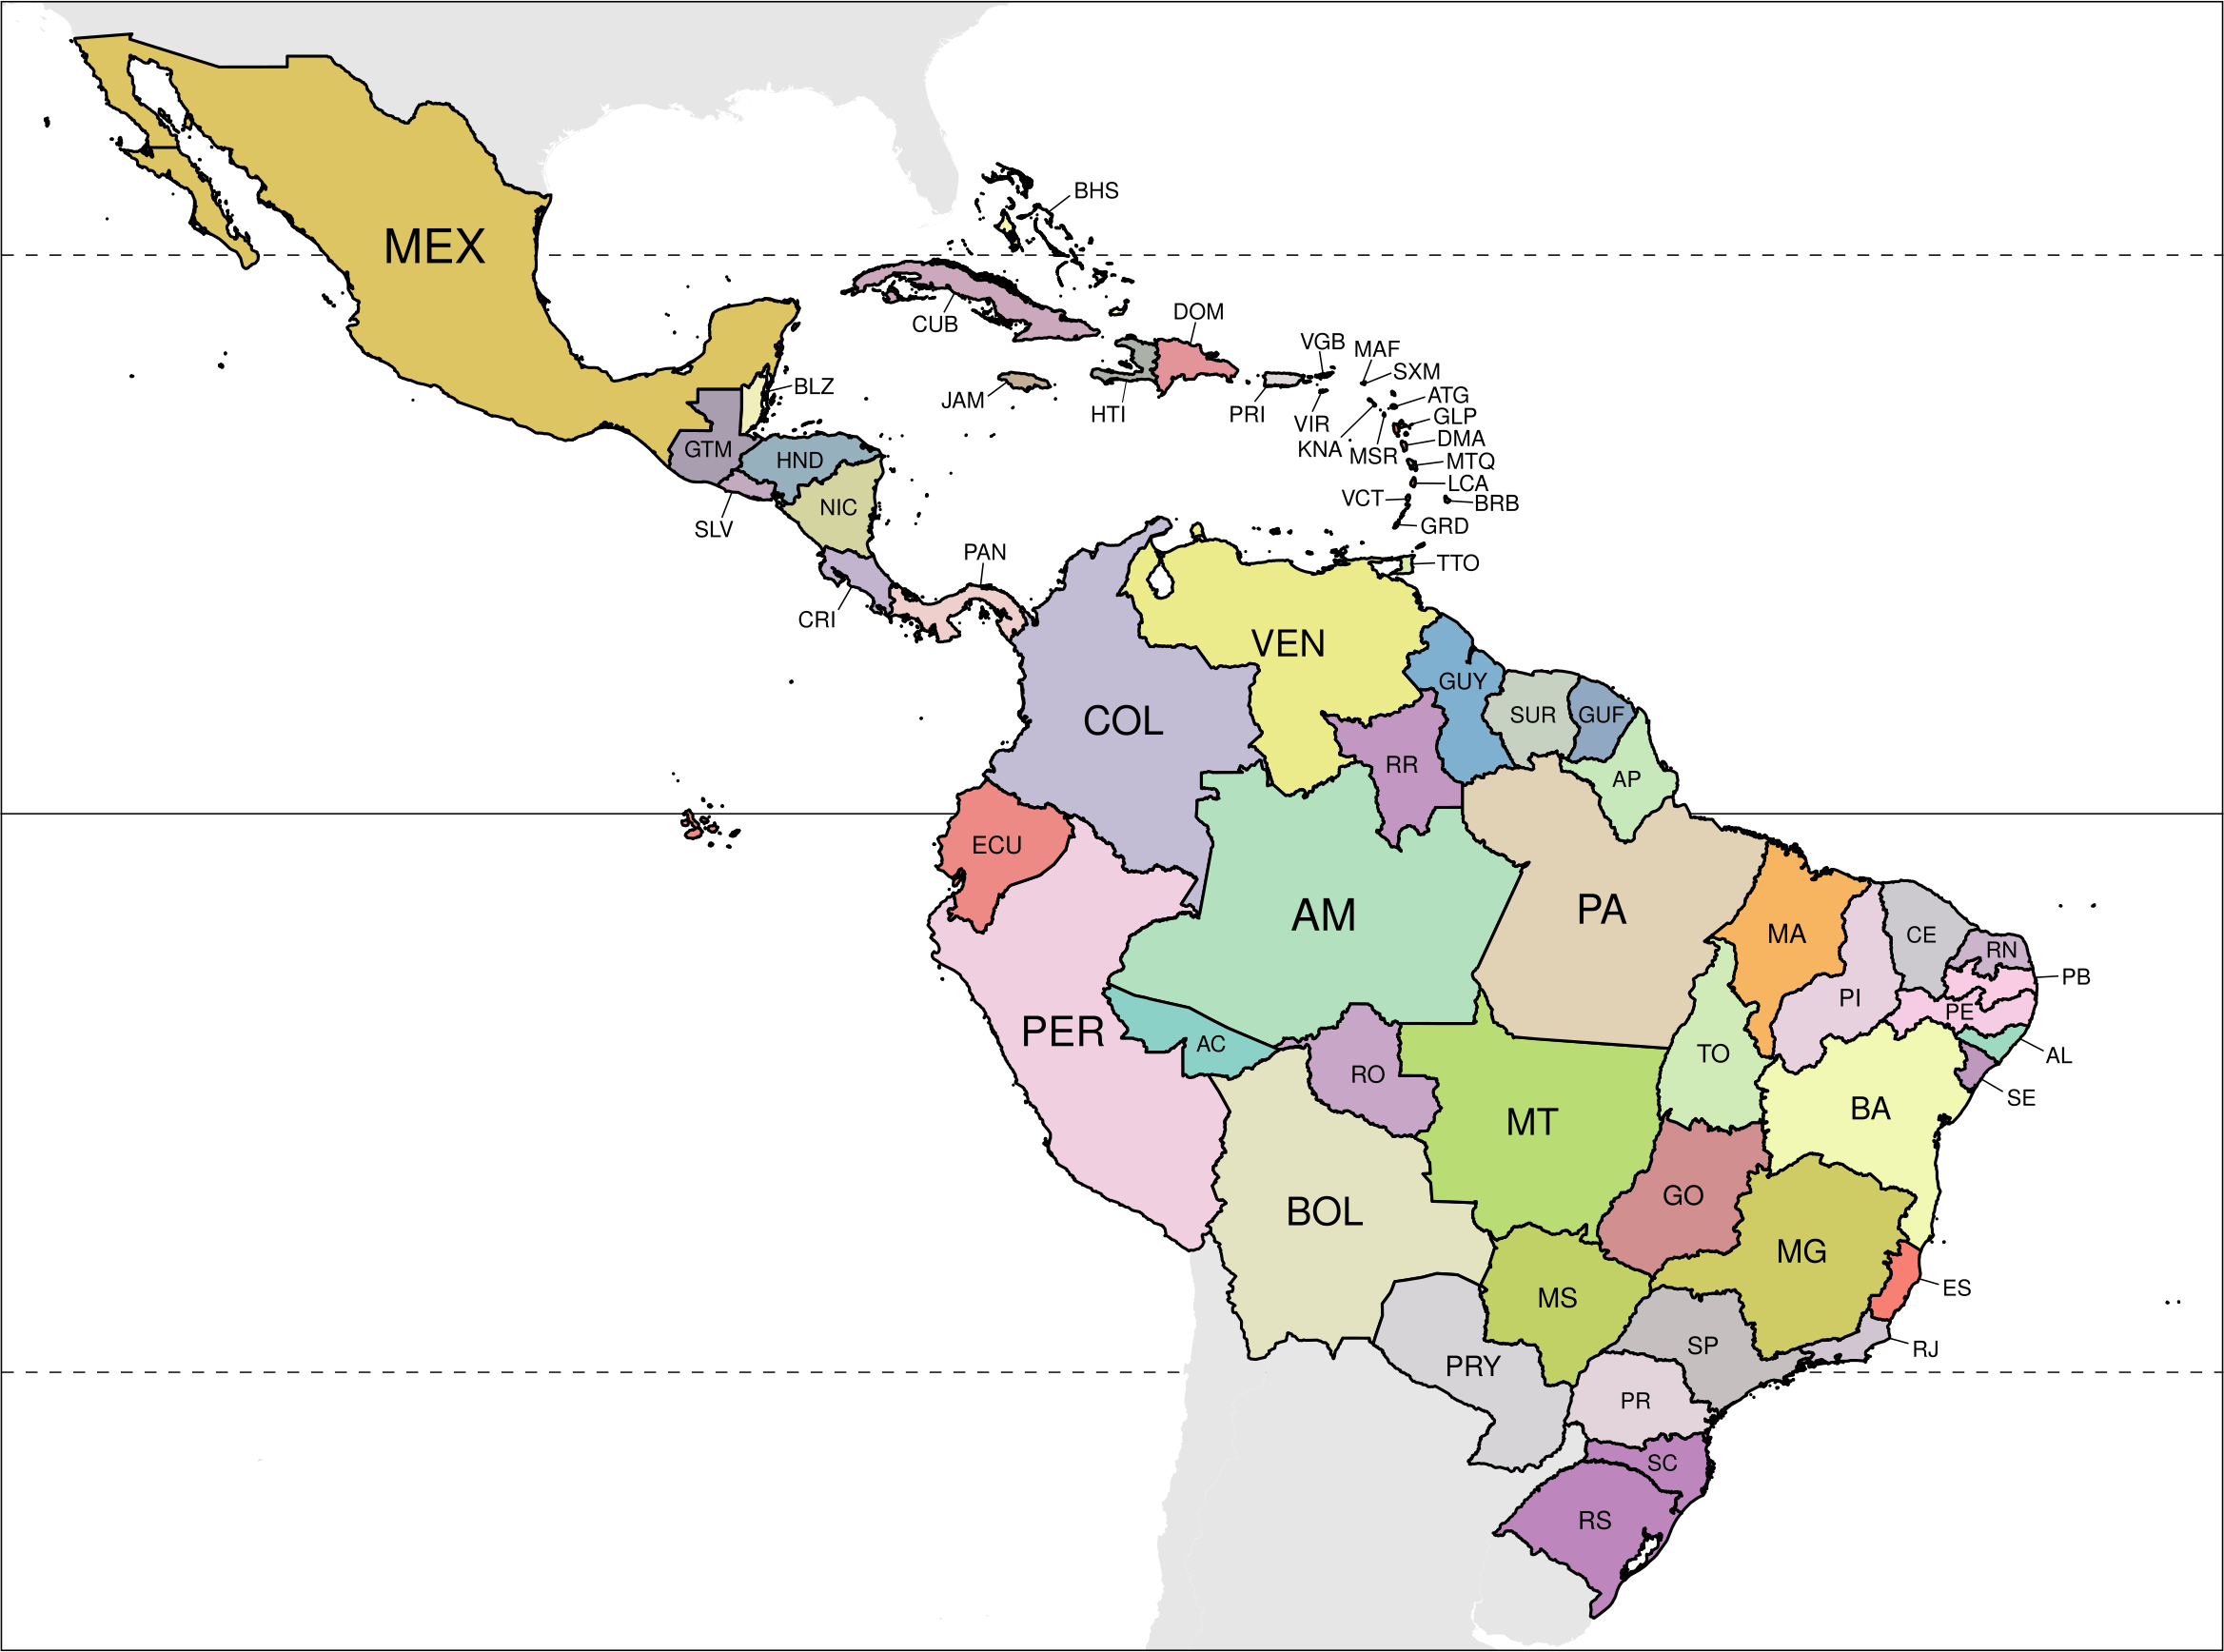
\includegraphics[width=0.32\textwidth]{figs/sm/study_areas_America}
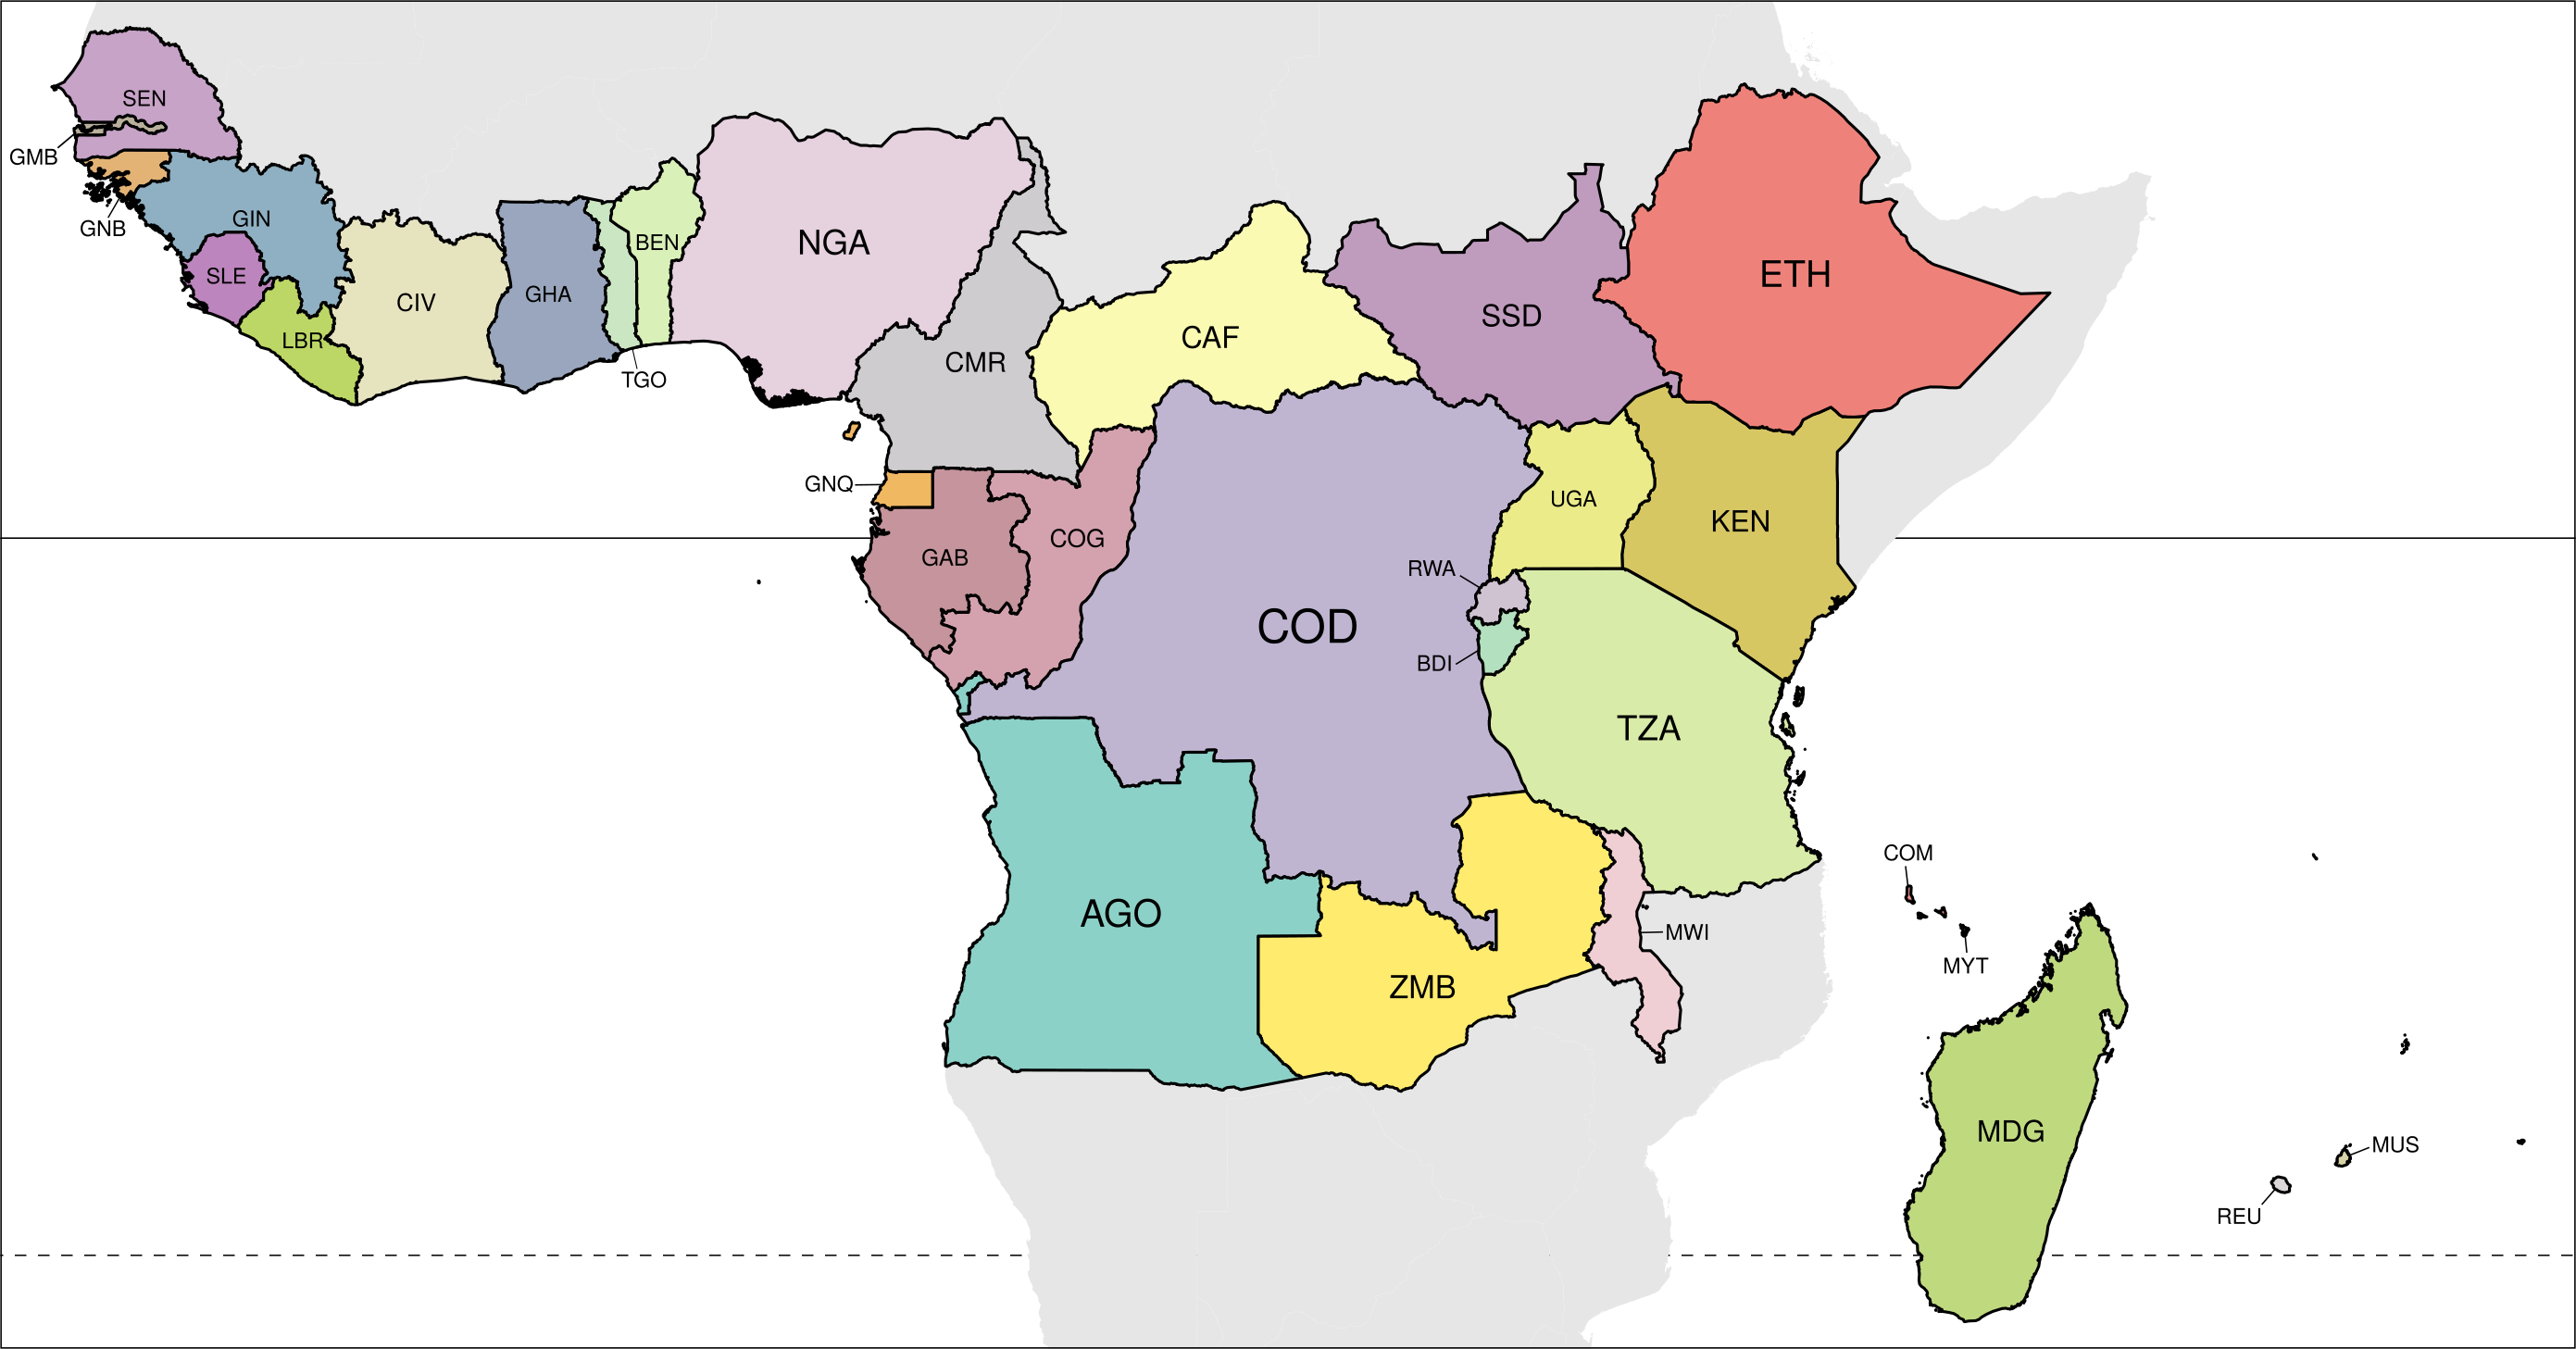
\includegraphics[width=0.32\textwidth]{figs/sm/study_areas_Africa}
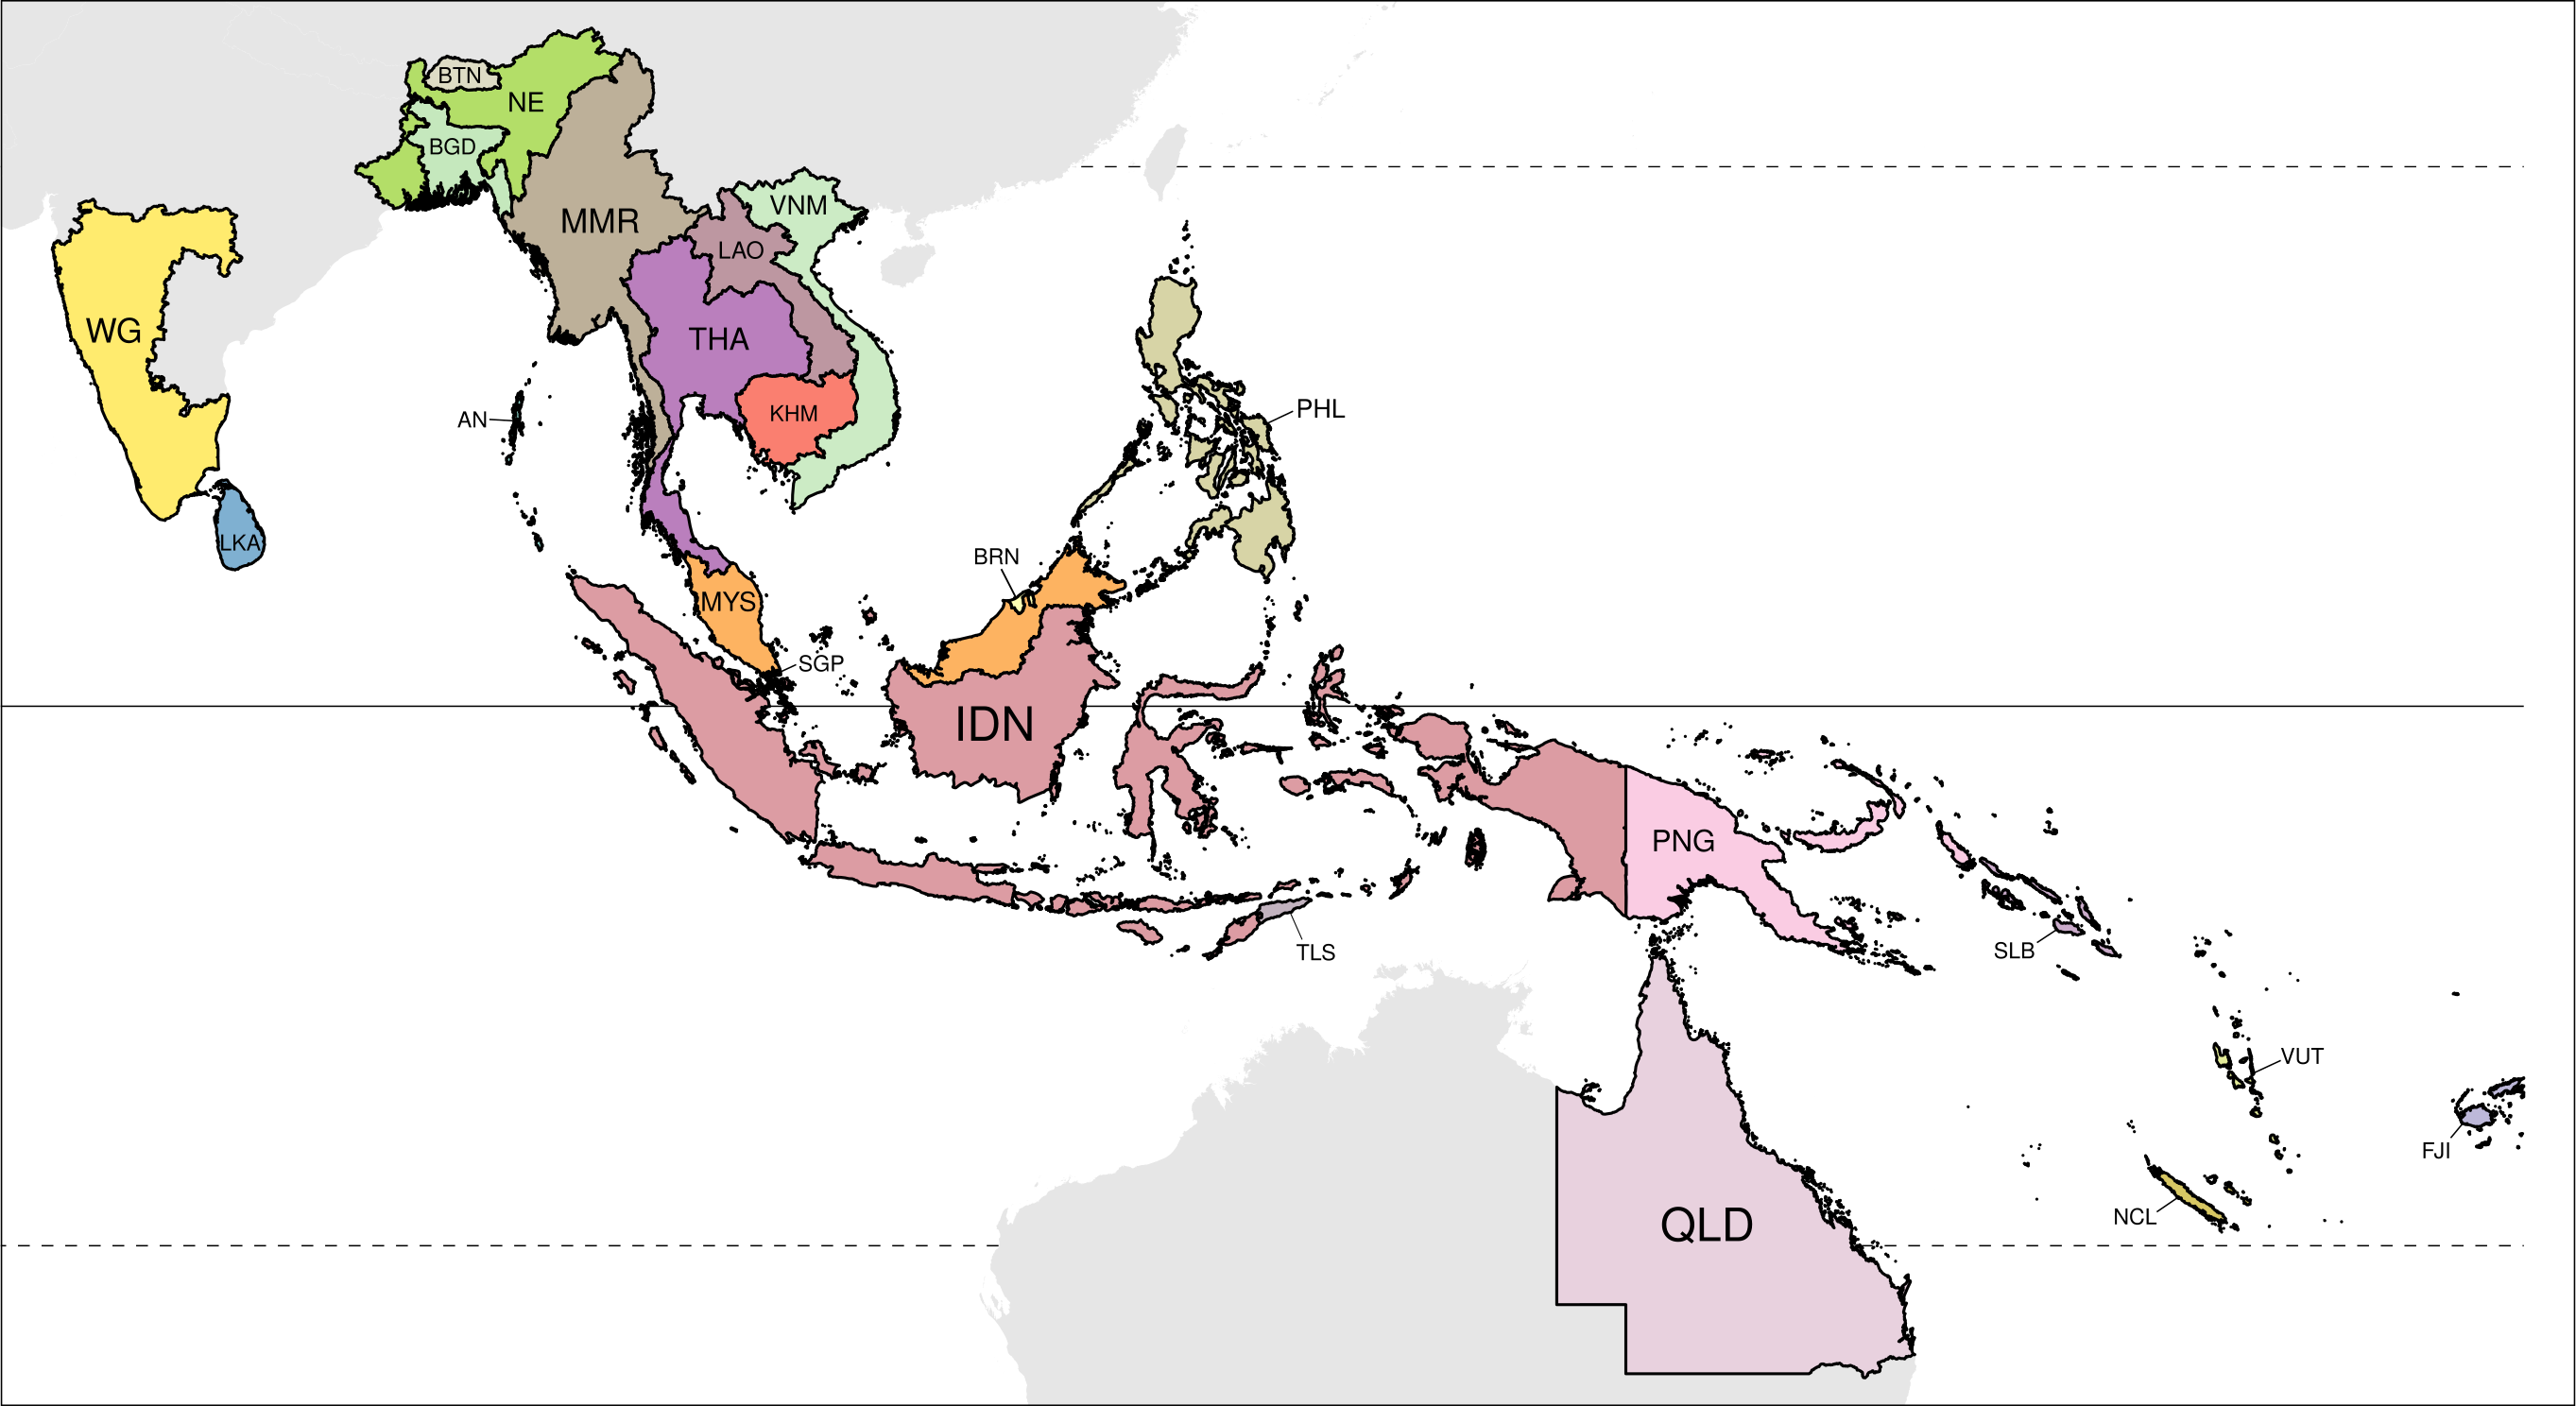
\includegraphics[width=0.32\textwidth]{figs/sm/study_areas_Asia}
\textbf{Las 119 zonas de estudio en los 3 continentes}
\end{center}
\end{frame}

\begin{frame}[label={sec:org0624b06}]{ForestAtRisk en los trópicos}
\begin{center}
\includegraphics[width=0.7\textwidth]{figs/article/prob.png}
\end{center}

\textbf{Mapa pantropical de la probabilidad espacial de deforestación}

Artículo en revisión:
\href{https://doi.org/10.1101/2022.03.22.485306}{10.1101/2022.03.22.485306}

\url{https://forestatrisk.cirad.fr/maps.html}
\end{frame}

\subsection{Modelos de ventanas móviles}
\label{sec:orgbbb3a86}

\begin{frame}[label={sec:orgd351244}]{Modelos de ventanas móviles}
\begin{itemize}
\item Modelo propuesto por la anterior metodología de Verra.
\item Encontrar un umbral de distancia para definir la clase 1 para el riesgo de
deforestación (lo mismo que para el modelo de referencia).
\end{itemize}

\begin{columns}
\begin{column}{0.55\columnwidth}
\begin{figure}[htbp]
\centering
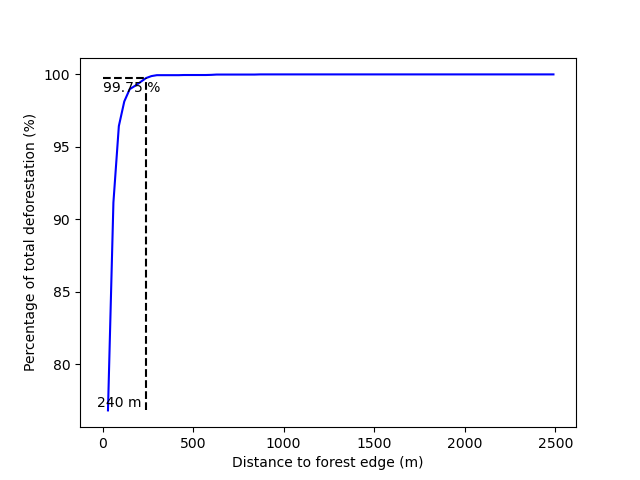
\includegraphics[width=\textwidth]{figs/get_started/perc_dist.png}
\caption{Deforestación acumulada en función de la distancia al borde del bosque.}
\end{figure}
\end{column}

\begin{column}{0.45\columnwidth}
\begin{center}
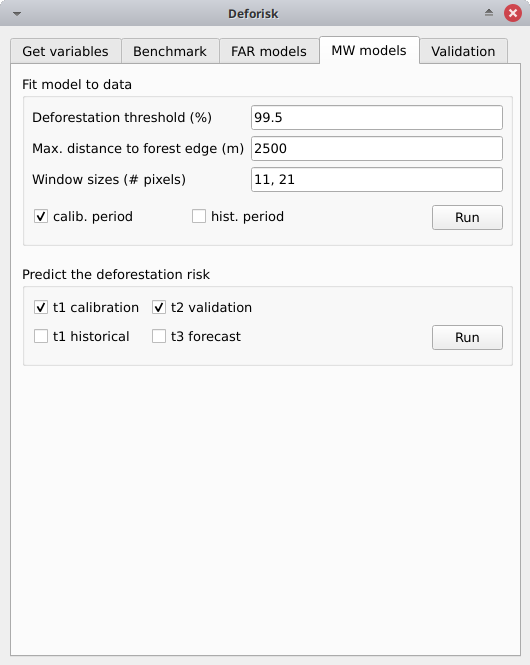
\includegraphics[width=0.9\textwidth]{figs/plugin_api/interface_mw_models.png}
\end{center}
\end{column}
\end{columns}
\end{frame}

\begin{frame}[label={sec:org97be5e1}]{Modelos de ventanas móviles}
\begin{itemize}
\item Calcular un riesgo local de deforestación a nivel de píxel utilizando una
ventana móvil.
\item La ventana móvil puede ser de distintos tamaños.
\item Las tasas de deforestación en [0, 1] se convierten a [2, 65535].
\end{itemize}

\begin{figure}[htbp]
\centering
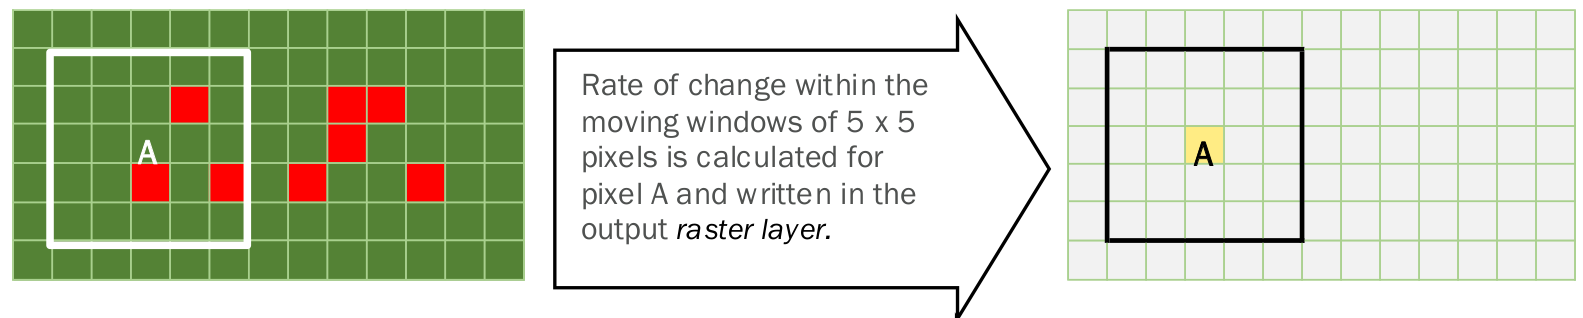
\includegraphics[width=0.8\textwidth]{figs/moving_window.png}
\caption{Ventana móvil.}
\end{figure}
\end{frame}

\subsection{Validación}
\label{sec:org384bc69}

\begin{frame}[label={sec:org2b0ec9c}]{Validación}
\begin{columns}
\begin{column}{0.5\columnwidth}
\begin{itemize}
\item Comparación de la deforestación prevista frente a la observada (en ha) para
cada celda de una cuadrícula gruesa.
\item Durante un periodo de tiempo determinado.
\end{itemize}
\begin{center}
\includegraphics[width=0.7\textwidth]{figs/grid.png}
\end{center}  
\end{column}
\begin{column}{0.5\columnwidth}
\begin{center}
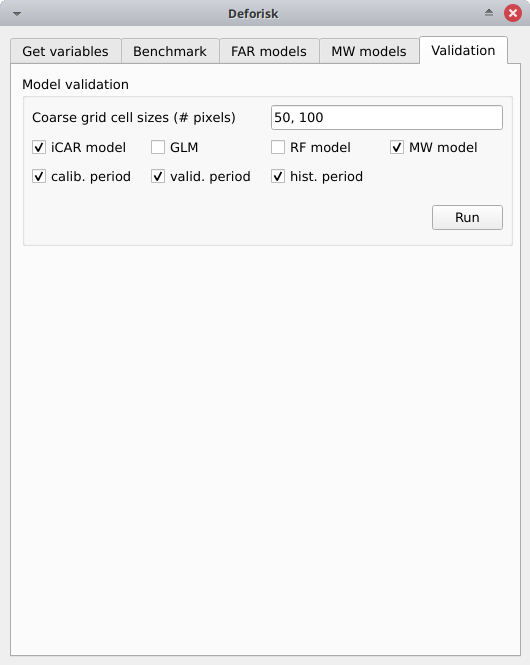
\includegraphics[width=\textwidth]{figs/plugin_api/interface_validation.png}
\end{center}
\end{column}
\end{columns}
\end{frame}

\begin{frame}[label={sec:org3609995}]{Validación}
\begin{itemize}
\item Índices de rendimiento: \(R^2\), y mediana del error absoluto (MedAE).
\item Calculados para cada modelo y cada periodo (calibración, validación,
histórico).
\end{itemize}

\begin{center}
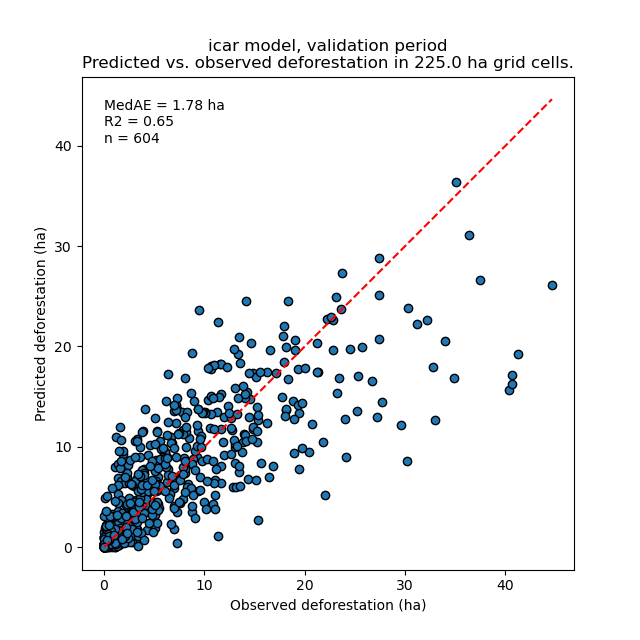
\includegraphics[width=0.6\textwidth]{figs/get_started/pred_obs_icar_validation_50.png}
\end{center}
\end{frame}

\section{Utilización}
\label{sec:org3edfc8e}

\subsection{Asignación de la deforestación}
\label{sec:org9fb3dab}

\begin{frame}[label={sec:orgff8474c}]{Asignación de la deforestación}
Para el mejor modelo, obtenemos en t3:
\begin{itemize}
\item Mapa jurisdiccional con clases de riesgo de deforestación.
\item Una tabla con las tasas relativas de deforestación de cada clase.
\end{itemize}

\begin{table}[htbp]
\caption{\label{tab-defrate}Tasas de deforestación en t3 para cada clase de riesgo de deforestación
(cifras truncadas a tres dígitos decimales).}
\small
\begin{tabular}{rrlrllrl}
\toprule cat & \(n_i\) & \(d_i\) & \(\theta_{m,i}\) & \(\theta_{a,i}\) & \(T\) & \(A\) & \(\delta_{i}\)\\[0pt] \midrule 1 & 137575 & -- & 1.000e-06 & -- & -- & 0.09 & --\\[0pt] 2 & 5425 & -- & 1.625e-05 & -- & -- & 0.09 & --\\[0pt] 3 & 3523 & -- & 3.151e-05 & -- & -- & 0.09 & --\\[0pt] 4 & 2458 & -- & 4.677e-05 & -- & -- & 0.09 & --\\[0pt] 5 & 2078 & -- & 6.203 & -- & -- & 0.09 & --\\[0pt] \bottomrule
\end{tabular}
\end{table}
\end{frame}

\begin{frame}[label={sec:org6aa68e5}]{Asignación de la deforestación}
\begin{table}[htbp]
\caption{\label{tab-defrate-header}Tasas de deforestación en t3 para cada clase de riesgo de deforestación
(cifras truncadas a tres dígitos decimales).}
\small
\begin{tabular}{rrlrllrl}
\toprule cat & \(n_i\) & \(d_i\) & \(\theta_{m,i}\) & \(\theta_{a,i}\) & \(T\) & \(A\) & \(\delta_{i}\)\\[0pt] \midrule 1 & 137575 & -- & 1.000e-06 & -- & -- & 0.09 & --\\[0pt] \bottomrule
\end{tabular}
\end{table}

\begin{itemize}
\item Considerando un total de \textbf{deforestación} \(D\) (en ha) para los
próximos \(Y\) \textbf{años} a nivel jurisdiccional.
\item \textbf{Factor de ajuste} es \(\rho = D / (A \sum_i n_{i} \theta_{m,i})\),
siendo \(A\) el área del píxel en ha.
\item \textbf{Tasa absoluta} es \(\theta_{a,i} = \rho \theta_{m,i}\): de modo que
deforestación total = deforestación prevista por los datos de actividad.
\item \textbf{Densidad de deforestación} es \(\delta_{i} = \theta_{a,i} \times A /
Y\). Se utiliza para predecir la cantidad de deforestación (en ha/año) de
cada píxel forestal.
\end{itemize}
\end{frame}

\begin{frame}[label={sec:orge68269d}]{Asignación de la deforestación}
\textbf{Densidad de deforestación} es \(\delta_{i} = \theta_{a,i} \times A /
Y\). Se utiliza para predecir la cantidad de deforestación (en ha/año) de
cada píxel forestal.

\begin{figure}[htbp]
\centering
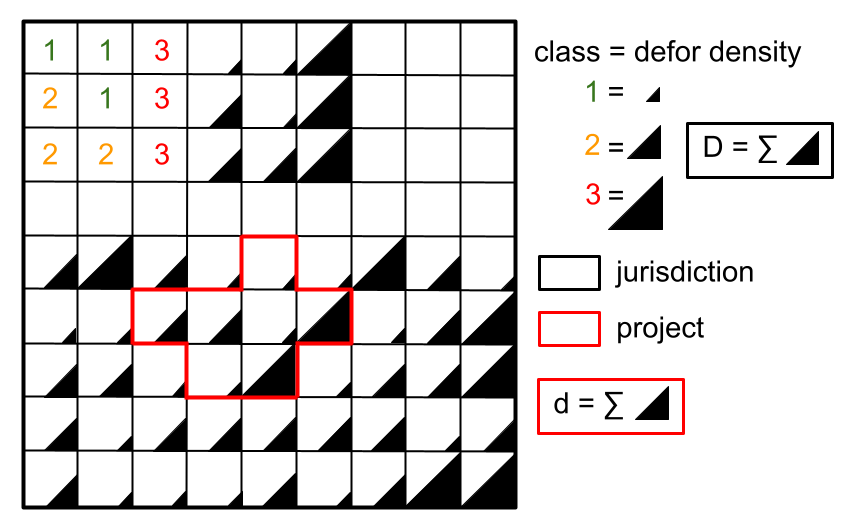
\includegraphics[width=8cm]{figs/get_started/allocation.png}
\caption{Asignación de la deforestación a proyectos dentro de la jurisdicción.}
\end{figure}
\end{frame}

\subsection{Jurisdicciones subnacionales}
\label{sec:orgada2c1e}

\begin{frame}[label={sec:org6424960},fragile]{Jurisdicciones subnacionales}
 \begin{itemize}
\item Posibilidad de trabajar con jurisdicciones subnacionales.
\item Archivo GPKG llamado \texttt{aoi\_latlon.gpkg} con dos capas llamadas
\texttt{aoi} para la jurisdicción y \texttt{subj} para las
subjurisdicciones.
\item Este archivo se puede utilizar con el plugin \texttt{deforisk} para definir
el área de interés (AOI).
\item Más información en la página web
\href{https://deforisk-qgis-plugin.org/es/articles/subnational\_jurisd.html}{Jurisdicciones
subnacionales}.
\end{itemize}

\begin{center}
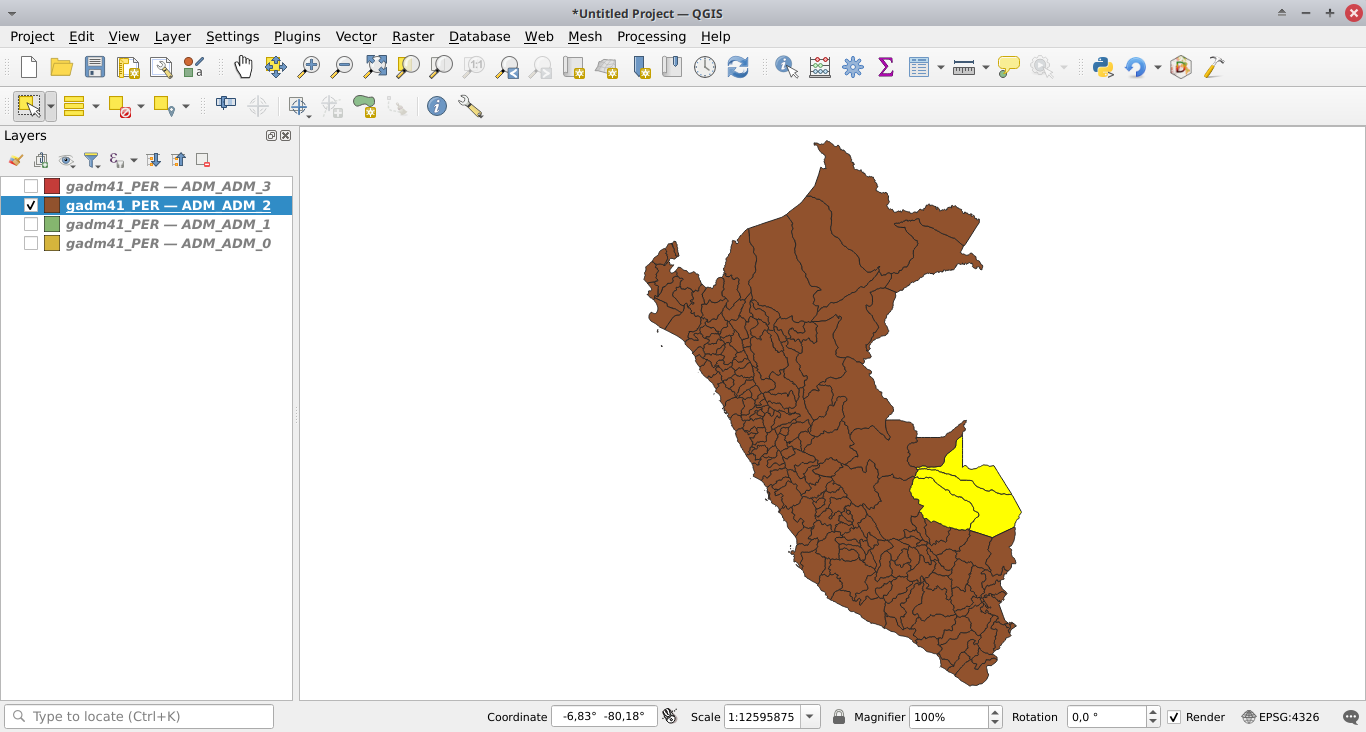
\includegraphics[width=7cm]{figs/select_subjurisdictions.png}
\end{center}
\end{frame}

\subsection{Datos del usuario}
\label{sec:org6992bcf}

\begin{frame}[label={sec:orgd079d9f},fragile]{Datos del usuario}
 \begin{itemize}
\item Posibilidad de utilizar datos del usuario: mapa nacional de cambios en la
cubierta forestal, otras variables explicativas (por ejemplo, concesiones
mineras).
\item Pasos manuales por el momento.
\item Los archivos de la carpeta \texttt{data} deben ser reemplazados por los
datos del usuario.
\item Se pueden añadir variables raster adicionales a la carpeta \texttt{data}.
\item Deben existir enlaces simbólicos en las carpetas \texttt{data\_*}.
\item Más detalles en la página web
\href{https://deforisk-qgis-plugin.org/es/articles/user\_data.html}{Datos
del usuario}.
\end{itemize}
\end{frame}

\section{Conclusión}
\label{sec:org8b1578c}

\subsection{Programa del taller}
\label{sec:org9e257b5}

\begin{frame}[label={sec:orgc45bd60},fragile]{Programa del taller}
 Cuatro sesiones prácticas:

\begin{itemize}
\item Instalar el software y ejecutar el tutorial \texttt{Get Started}.
\item Elegir una jurisdicción subnacional pequeña y seleccione el mejor mapa de
riesgos.
\item Derivar el mejor mapa de riesgos para una gran jurisdicción (por ejemplo, a
nivel nacional).
\item Ejercicios:
\begin{itemize}
\item Cambiar los parámetros del modelo para ver su comportamiento (por ejemplo,
el tamaño de las celdas espaciales para el modelo iCAR).
\item Utilizar datos del país (por ejemplo, mapa nacional de cambios en la
cubierta forestal).
\item Asignar la deforestación futura a un proyecto.
\end{itemize}
\end{itemize}
\end{frame}

\subsection{Perspectivas}
\label{sec:org679384f}

\begin{frame}[label={sec:org1c4e543}]{Perspectivas}
\begin{itemize}
\item Plugin reciente (primera versión en julio de 2024).
\item Se esperan mejoras:
\begin{itemize}
\item Aumentar la velocidad de cálculo (para predicciones sobre grandes
superficies).
\item Añadir más modelos alternativos (MLP).
\end{itemize}
\item Modificaciones a partir de los comentarios de los usuarios.
\end{itemize}
\end{frame}


{ \usebackgroundtemplate{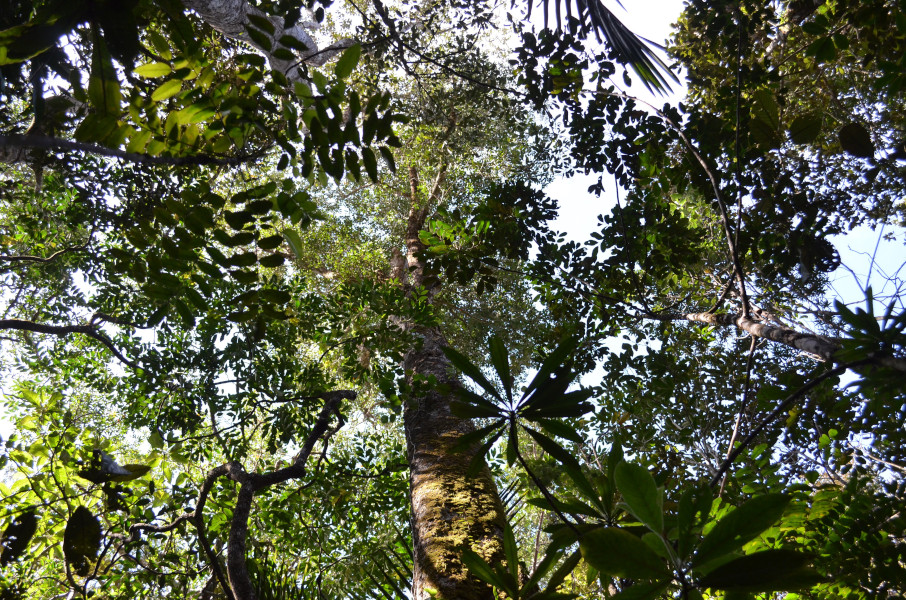
\includegraphics[keepaspectratio=true,
height=\paperheight]{figs/Canopy-NC} } \setbeamertemplate{navigation
symbols}{} \setbeamertemplate{blocks}[rounded][shadow=false]
\begin{frame}[plain] \vspace*{\stretch{100}} \begin{block}{} \begin{center}
\ldots~Gracias por su atención~\ldots \\ 
\url{https://deforisk-qgis-plugin.org} \\ \textbf{> Artículos > Referencias
> Presentaciones} \\ 

\includegraphics[width=0.8\textwidth]{figs/partners_logos} \end{center}
\end{block} \end{frame} }
\end{document}
